\documentclass[]{book}
\usepackage{lmodern}
\usepackage{amssymb,amsmath}
\usepackage{ifxetex,ifluatex}
\usepackage{fixltx2e} % provides \textsubscript
\ifnum 0\ifxetex 1\fi\ifluatex 1\fi=0 % if pdftex
  \usepackage[T1]{fontenc}
  \usepackage[utf8]{inputenc}
\else % if luatex or xelatex
  \ifxetex
    \usepackage{mathspec}
  \else
    \usepackage{fontspec}
  \fi
  \defaultfontfeatures{Ligatures=TeX,Scale=MatchLowercase}
\fi
% use upquote if available, for straight quotes in verbatim environments
\IfFileExists{upquote.sty}{\usepackage{upquote}}{}
% use microtype if available
\IfFileExists{microtype.sty}{%
\usepackage{microtype}
\UseMicrotypeSet[protrusion]{basicmath} % disable protrusion for tt fonts
}{}
\usepackage[margin=1in]{geometry}
\usepackage{hyperref}
\hypersetup{unicode=true,
            pdftitle={Linear Regression 202},
            pdfauthor={Alfonso R. Reyes},
            pdfborder={0 0 0},
            breaklinks=true}
\urlstyle{same}  % don't use monospace font for urls
\usepackage{natbib}
\bibliographystyle{apalike}
\usepackage{color}
\usepackage{fancyvrb}
\newcommand{\VerbBar}{|}
\newcommand{\VERB}{\Verb[commandchars=\\\{\}]}
\DefineVerbatimEnvironment{Highlighting}{Verbatim}{commandchars=\\\{\}}
% Add ',fontsize=\small' for more characters per line
\usepackage{framed}
\definecolor{shadecolor}{RGB}{248,248,248}
\newenvironment{Shaded}{\begin{snugshade}}{\end{snugshade}}
\newcommand{\AlertTok}[1]{\textcolor[rgb]{0.94,0.16,0.16}{#1}}
\newcommand{\AnnotationTok}[1]{\textcolor[rgb]{0.56,0.35,0.01}{\textbf{\textit{#1}}}}
\newcommand{\AttributeTok}[1]{\textcolor[rgb]{0.77,0.63,0.00}{#1}}
\newcommand{\BaseNTok}[1]{\textcolor[rgb]{0.00,0.00,0.81}{#1}}
\newcommand{\BuiltInTok}[1]{#1}
\newcommand{\CharTok}[1]{\textcolor[rgb]{0.31,0.60,0.02}{#1}}
\newcommand{\CommentTok}[1]{\textcolor[rgb]{0.56,0.35,0.01}{\textit{#1}}}
\newcommand{\CommentVarTok}[1]{\textcolor[rgb]{0.56,0.35,0.01}{\textbf{\textit{#1}}}}
\newcommand{\ConstantTok}[1]{\textcolor[rgb]{0.00,0.00,0.00}{#1}}
\newcommand{\ControlFlowTok}[1]{\textcolor[rgb]{0.13,0.29,0.53}{\textbf{#1}}}
\newcommand{\DataTypeTok}[1]{\textcolor[rgb]{0.13,0.29,0.53}{#1}}
\newcommand{\DecValTok}[1]{\textcolor[rgb]{0.00,0.00,0.81}{#1}}
\newcommand{\DocumentationTok}[1]{\textcolor[rgb]{0.56,0.35,0.01}{\textbf{\textit{#1}}}}
\newcommand{\ErrorTok}[1]{\textcolor[rgb]{0.64,0.00,0.00}{\textbf{#1}}}
\newcommand{\ExtensionTok}[1]{#1}
\newcommand{\FloatTok}[1]{\textcolor[rgb]{0.00,0.00,0.81}{#1}}
\newcommand{\FunctionTok}[1]{\textcolor[rgb]{0.00,0.00,0.00}{#1}}
\newcommand{\ImportTok}[1]{#1}
\newcommand{\InformationTok}[1]{\textcolor[rgb]{0.56,0.35,0.01}{\textbf{\textit{#1}}}}
\newcommand{\KeywordTok}[1]{\textcolor[rgb]{0.13,0.29,0.53}{\textbf{#1}}}
\newcommand{\NormalTok}[1]{#1}
\newcommand{\OperatorTok}[1]{\textcolor[rgb]{0.81,0.36,0.00}{\textbf{#1}}}
\newcommand{\OtherTok}[1]{\textcolor[rgb]{0.56,0.35,0.01}{#1}}
\newcommand{\PreprocessorTok}[1]{\textcolor[rgb]{0.56,0.35,0.01}{\textit{#1}}}
\newcommand{\RegionMarkerTok}[1]{#1}
\newcommand{\SpecialCharTok}[1]{\textcolor[rgb]{0.00,0.00,0.00}{#1}}
\newcommand{\SpecialStringTok}[1]{\textcolor[rgb]{0.31,0.60,0.02}{#1}}
\newcommand{\StringTok}[1]{\textcolor[rgb]{0.31,0.60,0.02}{#1}}
\newcommand{\VariableTok}[1]{\textcolor[rgb]{0.00,0.00,0.00}{#1}}
\newcommand{\VerbatimStringTok}[1]{\textcolor[rgb]{0.31,0.60,0.02}{#1}}
\newcommand{\WarningTok}[1]{\textcolor[rgb]{0.56,0.35,0.01}{\textbf{\textit{#1}}}}
\usepackage{longtable,booktabs}
\usepackage{graphicx,grffile}
\makeatletter
\def\maxwidth{\ifdim\Gin@nat@width>\linewidth\linewidth\else\Gin@nat@width\fi}
\def\maxheight{\ifdim\Gin@nat@height>\textheight\textheight\else\Gin@nat@height\fi}
\makeatother
% Scale images if necessary, so that they will not overflow the page
% margins by default, and it is still possible to overwrite the defaults
% using explicit options in \includegraphics[width, height, ...]{}
\setkeys{Gin}{width=\maxwidth,height=\maxheight,keepaspectratio}
\IfFileExists{parskip.sty}{%
\usepackage{parskip}
}{% else
\setlength{\parindent}{0pt}
\setlength{\parskip}{6pt plus 2pt minus 1pt}
}
\setlength{\emergencystretch}{3em}  % prevent overfull lines
\providecommand{\tightlist}{%
  \setlength{\itemsep}{0pt}\setlength{\parskip}{0pt}}
\setcounter{secnumdepth}{5}
% Redefines (sub)paragraphs to behave more like sections
\ifx\paragraph\undefined\else
\let\oldparagraph\paragraph
\renewcommand{\paragraph}[1]{\oldparagraph{#1}\mbox{}}
\fi
\ifx\subparagraph\undefined\else
\let\oldsubparagraph\subparagraph
\renewcommand{\subparagraph}[1]{\oldsubparagraph{#1}\mbox{}}
\fi

%%% Use protect on footnotes to avoid problems with footnotes in titles
\let\rmarkdownfootnote\footnote%
\def\footnote{\protect\rmarkdownfootnote}

%%% Change title format to be more compact
\usepackage{titling}

% Create subtitle command for use in maketitle
\providecommand{\subtitle}[1]{
  \posttitle{
    \begin{center}\large#1\end{center}
    }
}

\setlength{\droptitle}{-2em}

  \title{Linear Regression 202}
    \pretitle{\vspace{\droptitle}\centering\huge}
  \posttitle{\par}
    \author{Alfonso R. Reyes}
    \preauthor{\centering\large\emph}
  \postauthor{\par}
      \predate{\centering\large\emph}
  \postdate{\par}
    \date{2019-09-16}

\usepackage{booktabs}

\begin{document}
\maketitle

{
\setcounter{tocdepth}{1}
\tableofcontents
}
\hypertarget{prerequisites}{%
\chapter*{Prerequisites}\label{prerequisites}}
\addcontentsline{toc}{chapter}{Prerequisites}

This is a \emph{sample} book written in \textbf{Markdown}. You can use anything that Pandoc's Markdown supports, e.g., a math equation \(a^2 + b^2 = c^2\).

The \textbf{bookdown} package can be installed from CRAN or Github:

\begin{Shaded}
\begin{Highlighting}[]
\KeywordTok{install.packages}\NormalTok{(}\StringTok{"bookdown"}\NormalTok{)}
\CommentTok{# or the development version}
\CommentTok{# devtools::install_github("rstudio/bookdown")}
\end{Highlighting}
\end{Shaded}

Remember each Rmd file contains one and only one chapter, and a chapter is defined by the first-level heading \texttt{\#}.

To compile this example to PDF, you need XeLaTeX. You are recommended to install TinyTeX (which includes XeLaTeX): \url{https://yihui.name/tinytex/}.

\hypertarget{regression---cereals-dataset}{%
\chapter{Regression - cereals dataset}\label{regression---cereals-dataset}}

\hypertarget{introduction}{%
\section{Introduction}\label{introduction}}

Source: \url{https://www.analyticsvidhya.com/blog/2017/09/creating-visualizing-neural-network-in-r/}

Neural network is an information-processing machine and can be viewed as analogous to human nervous system. Just like human nervous system, which is made up of interconnected neurons, a neural network is made up of interconnected information processing units. The information processing units do not work in a linear manner. In fact, neural network draws its strength from parallel processing of information, which allows it to deal with non-linearity. Neural network becomes handy to infer meaning and detect patterns from complex data sets.

Neural network is considered as one of the most useful technique in the world of data analytics. However, it is complex and is often regarded as a black box, i.e.~users view the input and output of a neural network but remain clueless about the knowledge generating process. We hope that the article will help readers learn about the internal mechanism of a neural network and get hands-on experience to implement it in R.

\hypertarget{the-basics-of-neural-network}{%
\section{The Basics of Neural Network}\label{the-basics-of-neural-network}}

A neural network is a model characterized by an activation function, which is used by interconnected information processing units to transform input into output. A neural network has always been compared to human nervous system. Information in passed through interconnected units analogous to information passage through neurons in humans. The first layer of the neural network receives the raw input, processes it and passes the processed information to the hidden layers. The hidden layer passes the information to the last layer, which produces the output. The advantage of neural network is that it is adaptive in nature. It learns from the information provided, i.e.~trains itself from the data, which has a known outcome and optimizes its weights for a better prediction in situations with unknown outcome.

A perceptron, viz. single layer neural network, is the most basic form of a neural network. A perceptron receives multidimensional input and processes it using a weighted summation and an activation function. It is trained using a labeled data and learning algorithm that optimize the weights in the summation processor. A major limitation of perceptron model is its inability to deal with non-linearity. A multilayered neural network overcomes this limitation and helps solve non-linear problems. The input layer connects with hidden layer, which in turn connects to the output layer. The connections are weighted and weights are optimized using a learning rule.

There are many learning rules that are used with neural network:

\begin{enumerate}
\def\labelenumi{\alph{enumi})}
\tightlist
\item
  least mean square;
\item
  gradient descent;
\item
  newton's rule;
\item
  conjugate gradient etc.
\end{enumerate}

The learning rules can be used in conjunction with backpropgation error method. The learning rule is used to calculate the error at the output unit. This error is backpropagated to all the units such that the error at each unit is proportional to the contribution of that unit towards total error at the output unit. The errors at each unit are then used to optimize the weight at each connection. Figure 1 displays the structure of a simple neural network model for better understanding.

\hypertarget{fitting-neural-network-in-r}{%
\section{Fitting Neural Network in R}\label{fitting-neural-network-in-r}}

Now we will fit a neural network model in R. In this article, we use a subset of cereal dataset shared by Carnegie Mellon University (CMU). The details of the dataset are on the following link: \url{http://lib.stat.cmu.edu/DASL/Datafiles/Cereals.html}. The objective is to predict rating of the cereals variables such as calories, proteins, fat etc. The R script is provided side by side and is commented for better understanding of the user. . The data is in .csv format and can be downloaded by clicking: cereals.

Please set working directory in R using setwd( ) function, and keep cereal.csv in the working directory. We use rating as the dependent variable and calories, proteins, fat, sodium and fiber as the independent variables. We divide the data into training and test set. Training set is used to find the relationship between dependent and independent variables while the test set assesses the performance of the model. We use 60\% of the dataset as training set. The assignment of the data to training and test set is done using random sampling. We perform random sampling on R using sample ( ) function. We have used set.seed( ) to generate same random sample everytime and maintain consistency. We will use the index variable while fitting neural network to create training and test data sets. The R script is as follows:

\begin{Shaded}
\begin{Highlighting}[]
\CommentTok{## Creating index variable }

\CommentTok{# Read the Data}
\NormalTok{data =}\StringTok{ }\KeywordTok{read.csv}\NormalTok{(}\KeywordTok{file.path}\NormalTok{(data_raw_dir, }\StringTok{"cereals.csv"}\NormalTok{), }\DataTypeTok{header=}\NormalTok{T)}

\CommentTok{# Random sampling}
\NormalTok{samplesize =}\StringTok{ }\FloatTok{0.60} \OperatorTok{*}\StringTok{ }\KeywordTok{nrow}\NormalTok{(data)}
\KeywordTok{set.seed}\NormalTok{(}\DecValTok{80}\NormalTok{)}
\NormalTok{index =}\StringTok{ }\KeywordTok{sample}\NormalTok{( }\KeywordTok{seq_len}\NormalTok{ ( }\KeywordTok{nrow}\NormalTok{ ( data ) ), }\DataTypeTok{size =}\NormalTok{ samplesize )}

\CommentTok{# Create training and test set  }
\NormalTok{datatrain =}\StringTok{ }\NormalTok{data[ index, ]}
\NormalTok{datatest =}\StringTok{ }\NormalTok{data[ }\OperatorTok{-}\NormalTok{index, ]}
\end{Highlighting}
\end{Shaded}

\begin{Shaded}
\begin{Highlighting}[]
\NormalTok{dplyr}\OperatorTok{::}\KeywordTok{glimpse}\NormalTok{(data)}
\CommentTok{#> Observations: 75}
\CommentTok{#> Variables: 6}
\CommentTok{#> $ calories <int> 70, 120, 70, 50, 110, 110, 130, 90, 90, 120, 110, 120...}
\CommentTok{#> $ protein  <int> 4, 3, 4, 4, 2, 2, 3, 2, 3, 1, 6, 1, 3, 1, 2, 2, 1, 1,...}
\CommentTok{#> $ fat      <int> 1, 5, 1, 0, 2, 0, 2, 1, 0, 2, 2, 3, 2, 1, 0, 0, 0, 1,...}
\CommentTok{#> $ sodium   <int> 130, 15, 260, 140, 180, 125, 210, 200, 210, 220, 290,...}
\CommentTok{#> $ fiber    <dbl> 10.0, 2.0, 9.0, 14.0, 1.5, 1.0, 2.0, 4.0, 5.0, 0.0, 2...}
\CommentTok{#> $ rating   <dbl> 68.4, 34.0, 59.4, 93.7, 29.5, 33.2, 37.0, 49.1, 53.3,...}
\end{Highlighting}
\end{Shaded}

Now we fit a neural network on our data. We use neuralnet library for the analysis. The first step is to scale the cereal dataset. The scaling of data is essential because otherwise a variable may have large impact on the prediction variable only because of its scale. Using unscaled may lead to meaningless results. The common techniques to scale data are: min-max normalization, Z-score normalization, median and MAD, and tan-h estimators. The min-max normalization transforms the data into a common range, thus removing the scaling effect from all the variables. Unlike Z-score normalization and median and MAD method, the min-max method retains the original distribution of the variables. We use min-max normalization to scale the data. The R script for scaling the data is as follows.

\begin{Shaded}
\begin{Highlighting}[]
\CommentTok{## Scale data for neural network}

\NormalTok{max =}\StringTok{ }\KeywordTok{apply}\NormalTok{(data , }\DecValTok{2}\NormalTok{ , max)}
\NormalTok{min =}\StringTok{ }\KeywordTok{apply}\NormalTok{(data, }\DecValTok{2}\NormalTok{ , min)}
\NormalTok{scaled =}\StringTok{ }\KeywordTok{as.data.frame}\NormalTok{(}\KeywordTok{scale}\NormalTok{(data, }\DataTypeTok{center =}\NormalTok{ min, }\DataTypeTok{scale =}\NormalTok{ max }\OperatorTok{-}\StringTok{ }\NormalTok{min))}
\end{Highlighting}
\end{Shaded}

\begin{Shaded}
\begin{Highlighting}[]
\CommentTok{## Fit neural network }

\CommentTok{# install library}
\CommentTok{# install.packages("neuralnet ")}

\CommentTok{# load library}
\KeywordTok{library}\NormalTok{(neuralnet)}

\CommentTok{# creating training and test set}
\NormalTok{trainNN =}\StringTok{ }\NormalTok{scaled[index , ]}
\NormalTok{testNN =}\StringTok{ }\NormalTok{scaled[}\OperatorTok{-}\NormalTok{index , ]}

\CommentTok{# fit neural network}
\KeywordTok{set.seed}\NormalTok{(}\DecValTok{2}\NormalTok{)}
\NormalTok{NN =}\StringTok{ }\KeywordTok{neuralnet}\NormalTok{(rating }\OperatorTok{~}\StringTok{ }\NormalTok{calories }\OperatorTok{+}\StringTok{ }\NormalTok{protein }\OperatorTok{+}\StringTok{ }\NormalTok{fat }\OperatorTok{+}\StringTok{ }\NormalTok{sodium }\OperatorTok{+}\StringTok{ }\NormalTok{fiber, }
\NormalTok{               trainNN, }\DataTypeTok{hidden =} \DecValTok{3}\NormalTok{ , }\DataTypeTok{linear.output =}\NormalTok{ T )}

\CommentTok{# plot neural network}
\KeywordTok{plot}\NormalTok{(NN)}
\end{Highlighting}
\end{Shaded}

\begin{Shaded}
\begin{Highlighting}[]
\CommentTok{## Prediction using neural network}

\NormalTok{predict_testNN =}\StringTok{ }\KeywordTok{compute}\NormalTok{(NN, testNN[,}\KeywordTok{c}\NormalTok{(}\DecValTok{1}\OperatorTok{:}\DecValTok{5}\NormalTok{)])}
\NormalTok{predict_testNN =}\StringTok{ }\NormalTok{(predict_testNN}\OperatorTok{$}\NormalTok{net.result }\OperatorTok{*}\StringTok{ }\NormalTok{(}\KeywordTok{max}\NormalTok{(data}\OperatorTok{$}\NormalTok{rating) }\OperatorTok{-}\StringTok{ }\KeywordTok{min}\NormalTok{(data}\OperatorTok{$}\NormalTok{rating))) }\OperatorTok{+}\StringTok{ }\KeywordTok{min}\NormalTok{(data}\OperatorTok{$}\NormalTok{rating)}

\KeywordTok{plot}\NormalTok{(datatest}\OperatorTok{$}\NormalTok{rating, predict_testNN, }\DataTypeTok{col=}\StringTok{'blue'}\NormalTok{, }\DataTypeTok{pch=}\DecValTok{16}\NormalTok{, }\DataTypeTok{ylab =} \StringTok{"predicted rating NN"}\NormalTok{, }\DataTypeTok{xlab =} \StringTok{"real rating"}\NormalTok{)}

\KeywordTok{abline}\NormalTok{(}\DecValTok{0}\NormalTok{,}\DecValTok{1}\NormalTok{)}

\CommentTok{# Calculate Root Mean Square Error (RMSE)}
\NormalTok{RMSE.NN =}\StringTok{ }\NormalTok{(}\KeywordTok{sum}\NormalTok{((datatest}\OperatorTok{$}\NormalTok{rating }\OperatorTok{-}\StringTok{ }\NormalTok{predict_testNN)}\OperatorTok{^}\DecValTok{2}\NormalTok{) }\OperatorTok{/}\StringTok{ }\KeywordTok{nrow}\NormalTok{(datatest)) }\OperatorTok{^}\StringTok{ }\FloatTok{0.5}
\end{Highlighting}
\end{Shaded}

\begin{center}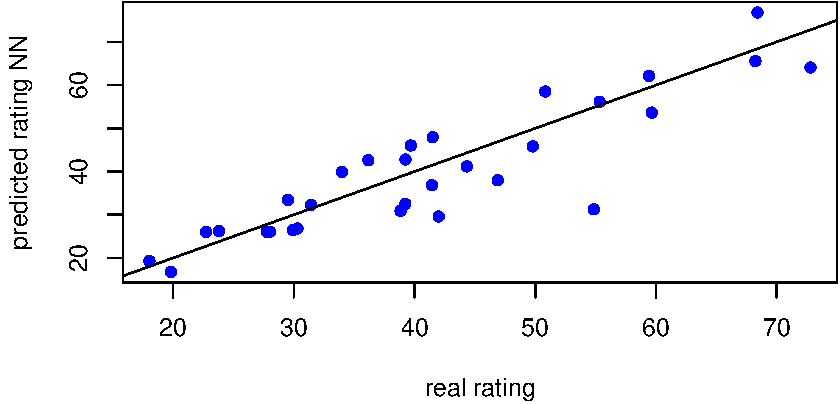
\includegraphics[width=0.7\linewidth]{regression_144-nn_cereals_neuralnet_files/figure-latex/predict_nn-1} \end{center}

\begin{Shaded}
\begin{Highlighting}[]
\CommentTok{## Cross validation of neural network model}

\CommentTok{# install relevant libraries}
\CommentTok{# install.packages("boot")}
\CommentTok{# install.packages("plyr")}

\CommentTok{# Load libraries}
\KeywordTok{library}\NormalTok{(boot)}
\KeywordTok{library}\NormalTok{(plyr)}

\CommentTok{# Initialize variables}
\KeywordTok{set.seed}\NormalTok{(}\DecValTok{50}\NormalTok{)}
\NormalTok{k =}\StringTok{ }\DecValTok{100}
\NormalTok{RMSE.NN =}\StringTok{ }\OtherTok{NULL}

\NormalTok{List =}\StringTok{ }\KeywordTok{list}\NormalTok{( )}

\CommentTok{# Fit neural network model within nested for loop}
\ControlFlowTok{for}\NormalTok{(j }\ControlFlowTok{in} \DecValTok{10}\OperatorTok{:}\DecValTok{65}\NormalTok{)\{}
    \ControlFlowTok{for}\NormalTok{ (i }\ControlFlowTok{in} \DecValTok{1}\OperatorTok{:}\NormalTok{k) \{}
\NormalTok{        index =}\StringTok{ }\KeywordTok{sample}\NormalTok{(}\DecValTok{1}\OperatorTok{:}\KeywordTok{nrow}\NormalTok{(data),j )}

\NormalTok{        trainNN =}\StringTok{ }\NormalTok{scaled[index,]}
\NormalTok{        testNN =}\StringTok{ }\NormalTok{scaled[}\OperatorTok{-}\NormalTok{index,]}
\NormalTok{        datatest =}\StringTok{ }\NormalTok{data[}\OperatorTok{-}\NormalTok{index,]}

\NormalTok{        NN =}\StringTok{ }\KeywordTok{neuralnet}\NormalTok{(rating }\OperatorTok{~}\StringTok{ }\NormalTok{calories }\OperatorTok{+}\StringTok{ }\NormalTok{protein }\OperatorTok{+}\StringTok{ }\NormalTok{fat }\OperatorTok{+}\StringTok{ }\NormalTok{sodium }\OperatorTok{+}\StringTok{ }\NormalTok{fiber, trainNN, }\DataTypeTok{hidden =} \DecValTok{3}\NormalTok{, }\DataTypeTok{linear.output=}\NormalTok{ T)}
\NormalTok{        predict_testNN =}\StringTok{ }\KeywordTok{compute}\NormalTok{(NN,testNN[,}\KeywordTok{c}\NormalTok{(}\DecValTok{1}\OperatorTok{:}\DecValTok{5}\NormalTok{)])}
\NormalTok{        predict_testNN =}\StringTok{ }\NormalTok{(predict_testNN}\OperatorTok{$}\NormalTok{net.result}\OperatorTok{*}\NormalTok{(}\KeywordTok{max}\NormalTok{(data}\OperatorTok{$}\NormalTok{rating)}\OperatorTok{-}\KeywordTok{min}\NormalTok{(data}\OperatorTok{$}\NormalTok{rating)))}\OperatorTok{+}\KeywordTok{min}\NormalTok{(data}\OperatorTok{$}\NormalTok{rating)}

\NormalTok{        RMSE.NN [i]<-}\StringTok{ }\NormalTok{(}\KeywordTok{sum}\NormalTok{((datatest}\OperatorTok{$}\NormalTok{rating }\OperatorTok{-}\StringTok{ }\NormalTok{predict_testNN)}\OperatorTok{^}\DecValTok{2}\NormalTok{)}\OperatorTok{/}\KeywordTok{nrow}\NormalTok{(datatest))}\OperatorTok{^}\FloatTok{0.5}
\NormalTok{    \}}
\NormalTok{    List[[j]] =}\StringTok{ }\NormalTok{RMSE.NN}
\NormalTok{\}}

\NormalTok{Matrix.RMSE =}\StringTok{ }\KeywordTok{do.call}\NormalTok{(cbind, List)}
\end{Highlighting}
\end{Shaded}

\begin{Shaded}
\begin{Highlighting}[]
\CommentTok{## Prepare boxplot}
\KeywordTok{boxplot}\NormalTok{(Matrix.RMSE[,}\DecValTok{56}\NormalTok{], }\DataTypeTok{ylab =} \StringTok{"RMSE"}\NormalTok{, }\DataTypeTok{main =} \StringTok{"RMSE BoxPlot (length of traning set = 65)"}\NormalTok{)}
\end{Highlighting}
\end{Shaded}

\begin{center}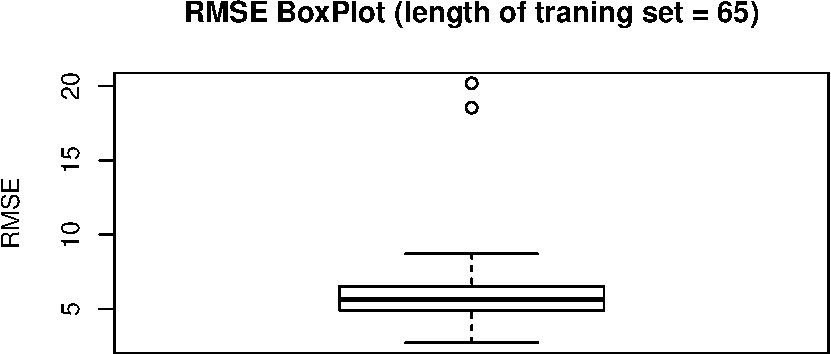
\includegraphics[width=0.7\linewidth]{regression_144-nn_cereals_neuralnet_files/figure-latex/boxplot-1} \end{center}



\begin{Shaded}
\begin{Highlighting}[]
\CommentTok{## Variation of median RMSE }
\CommentTok{# install.packages("matrixStats")}
\KeywordTok{library}\NormalTok{(matrixStats)}
\CommentTok{#> }
\CommentTok{#> Attaching package: 'matrixStats'}
\CommentTok{#> The following object is masked from 'package:plyr':}
\CommentTok{#> }
\CommentTok{#>     count}

\NormalTok{med =}\StringTok{ }\KeywordTok{colMedians}\NormalTok{(Matrix.RMSE)}

\NormalTok{X =}\StringTok{ }\KeywordTok{seq}\NormalTok{(}\DecValTok{10}\NormalTok{,}\DecValTok{65}\NormalTok{)}

\KeywordTok{plot}\NormalTok{ (med}\OperatorTok{~}\NormalTok{X, }\DataTypeTok{type =} \StringTok{"l"}\NormalTok{, }\DataTypeTok{xlab =} \StringTok{"length of training set"}\NormalTok{, }\DataTypeTok{ylab =} \StringTok{"median RMSE"}\NormalTok{, }\DataTypeTok{main =} \StringTok{"Variation of RMSE with length of training set"}\NormalTok{)}
\end{Highlighting}
\end{Shaded}

\begin{figure}

{\centering 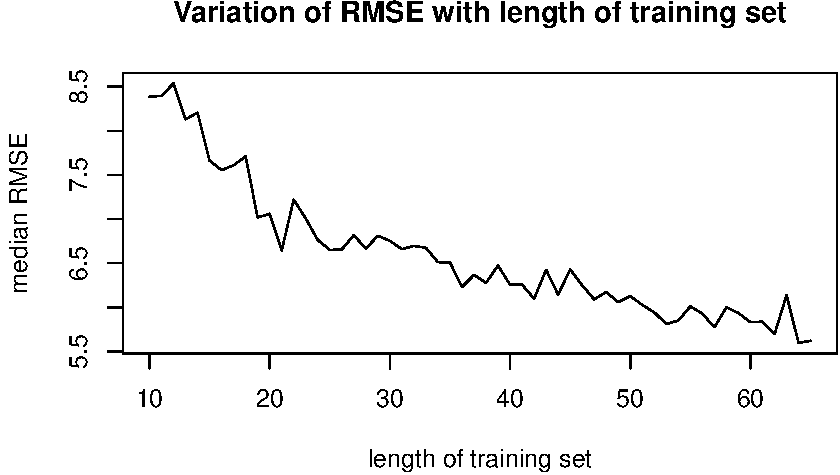
\includegraphics[width=0.7\linewidth]{regression_144-nn_cereals_neuralnet_files/figure-latex/var-rmse-1} 

}

\caption{Variation of RMSE}\label{fig:var-rmse}
\end{figure}

Figure \ref{fig:var-rmse}) shows that the median RMSE of our model decreases as the length of the training the set. This is an important result. The reader must remember that the model accuracy is dependent on the length of training set. The performance of neural network model is sensitive to training-test split.

\hypertarget{end-notes}{%
\section{End Notes}\label{end-notes}}

The article discusses the theoretical aspects of a neural network, its implementation in R and post training evaluation. Neural network is inspired from biological nervous system. Similar to nervous system the information is passed through layers of processors. The significance of variables is represented by weights of each connection. The article provides basic understanding of back propagation algorithm, which is used to assign these weights. In this article we also implement neural network on R. We use a publically available dataset shared by CMU. The aim is to predict the rating of cereals using information such as calories, fat, protein etc. After constructing the neural network we evaluate the model for accuracy and robustness. We compute RMSE and perform cross-validation analysis. In cross validation, we check the variation in model accuracy as the length of training set is changed. We consider training sets with length 10 to 65. For each length a 100 samples are random picked and median RMSE is calculated. We show that model accuracy increases when training set is large. Before using the model for prediction, it is important to check the robustness of performance through cross validation.

The article provides a quick review neural network and is a useful reference for data enthusiasts. We have provided commented R code throughout the article to help readers with hands on experience of using neural networks.

\hypertarget{fitting-a-neural-network}{%
\chapter{Fitting a neural network}\label{fitting-a-neural-network}}

\hypertarget{introduction-1}{%
\section{Introduction}\label{introduction-1}}

\url{https://www.r-bloggers.com/fitting-a-neural-network-in-r-neuralnet-package/}

\url{https://datascienceplus.com/fitting-neural-network-in-r/}

Neural networks have always been one of the fascinating machine learning models in my opinion, not only because of the fancy backpropagation algorithm but also because of their complexity (think of deep learning with many hidden layers) and structure inspired by the brain.

Neural networks have not always been popular, partly because they were, and still are in some cases, computationally expensive and partly because they did not seem to yield better results when compared with simpler methods such as support vector machines (SVMs). Nevertheless, Neural Networks have, once again, raised attention and become popular.

Update: We published another post about Network analysis at DataScience+ Network analysis of Game of Thrones

In this post, we are going to fit a simple neural network using the neuralnet package and fit a linear model as a comparison.

\hypertarget{the-dataset}{%
\section{The dataset}\label{the-dataset}}

We are going to use the Boston dataset in the MASS package.
The Boston dataset is a collection of data about housing values in the suburbs of Boston. Our goal is to predict the median value of owner-occupied homes (medv) using all the other continuous variables available.

\begin{Shaded}
\begin{Highlighting}[]
\KeywordTok{set.seed}\NormalTok{(}\DecValTok{500}\NormalTok{)}
\KeywordTok{library}\NormalTok{(MASS)}
\NormalTok{data <-}\StringTok{ }\NormalTok{Boston}
\end{Highlighting}
\end{Shaded}

\begin{Shaded}
\begin{Highlighting}[]
\NormalTok{dplyr}\OperatorTok{::}\KeywordTok{glimpse}\NormalTok{(data)}
\CommentTok{#> Observations: 506}
\CommentTok{#> Variables: 14}
\CommentTok{#> $ crim    <dbl> 0.00632, 0.02731, 0.02729, 0.03237, 0.06905, 0.02985, ...}
\CommentTok{#> $ zn      <dbl> 18.0, 0.0, 0.0, 0.0, 0.0, 0.0, 12.5, 12.5, 12.5, 12.5,...}
\CommentTok{#> $ indus   <dbl> 2.31, 7.07, 7.07, 2.18, 2.18, 2.18, 7.87, 7.87, 7.87, ...}
\CommentTok{#> $ chas    <int> 0, 0, 0, 0, 0, 0, 0, 0, 0, 0, 0, 0, 0, 0, 0, 0, 0, 0, ...}
\CommentTok{#> $ nox     <dbl> 0.538, 0.469, 0.469, 0.458, 0.458, 0.458, 0.524, 0.524...}
\CommentTok{#> $ rm      <dbl> 6.58, 6.42, 7.18, 7.00, 7.15, 6.43, 6.01, 6.17, 5.63, ...}
\CommentTok{#> $ age     <dbl> 65.2, 78.9, 61.1, 45.8, 54.2, 58.7, 66.6, 96.1, 100.0,...}
\CommentTok{#> $ dis     <dbl> 4.09, 4.97, 4.97, 6.06, 6.06, 6.06, 5.56, 5.95, 6.08, ...}
\CommentTok{#> $ rad     <int> 1, 2, 2, 3, 3, 3, 5, 5, 5, 5, 5, 5, 5, 4, 4, 4, 4, 4, ...}
\CommentTok{#> $ tax     <dbl> 296, 242, 242, 222, 222, 222, 311, 311, 311, 311, 311,...}
\CommentTok{#> $ ptratio <dbl> 15.3, 17.8, 17.8, 18.7, 18.7, 18.7, 15.2, 15.2, 15.2, ...}
\CommentTok{#> $ black   <dbl> 397, 397, 393, 395, 397, 394, 396, 397, 387, 387, 393,...}
\CommentTok{#> $ lstat   <dbl> 4.98, 9.14, 4.03, 2.94, 5.33, 5.21, 12.43, 19.15, 29.9...}
\CommentTok{#> $ medv    <dbl> 24.0, 21.6, 34.7, 33.4, 36.2, 28.7, 22.9, 27.1, 16.5, ...}
\end{Highlighting}
\end{Shaded}

First we need to check that no datapoint is missing, otherwise we need to fix the dataset.

\begin{Shaded}
\begin{Highlighting}[]
\KeywordTok{apply}\NormalTok{(data,}\DecValTok{2}\NormalTok{,}\ControlFlowTok{function}\NormalTok{(x) }\KeywordTok{sum}\NormalTok{(}\KeywordTok{is.na}\NormalTok{(x)))}
\CommentTok{#>    crim      zn   indus    chas     nox      rm     age     dis     rad }
\CommentTok{#>       0       0       0       0       0       0       0       0       0 }
\CommentTok{#>     tax ptratio   black   lstat    medv }
\CommentTok{#>       0       0       0       0       0}
\end{Highlighting}
\end{Shaded}

There is no missing data, good. We proceed by randomly splitting the data into a train and a test set, then we fit a linear regression model and test it on the test set. Note that I am using the gml() function instead of the lm() this will become useful later when cross validating the linear model.

\begin{Shaded}
\begin{Highlighting}[]
\NormalTok{index <-}\StringTok{ }\KeywordTok{sample}\NormalTok{(}\DecValTok{1}\OperatorTok{:}\KeywordTok{nrow}\NormalTok{(data),}\KeywordTok{round}\NormalTok{(}\FloatTok{0.75}\OperatorTok{*}\KeywordTok{nrow}\NormalTok{(data)))}
\NormalTok{train <-}\StringTok{ }\NormalTok{data[index,]}
\NormalTok{test <-}\StringTok{ }\NormalTok{data[}\OperatorTok{-}\NormalTok{index,]}
\NormalTok{lm.fit <-}\StringTok{ }\KeywordTok{glm}\NormalTok{(medv}\OperatorTok{~}\NormalTok{., }\DataTypeTok{data=}\NormalTok{train)}
\KeywordTok{summary}\NormalTok{(lm.fit)}
\CommentTok{#> }
\CommentTok{#> Call:}
\CommentTok{#> glm(formula = medv ~ ., data = train)}
\CommentTok{#> }
\CommentTok{#> Deviance Residuals: }
\CommentTok{#>     Min       1Q   Median       3Q      Max  }
\CommentTok{#> -15.211   -2.559   -0.655    1.828   29.711  }
\CommentTok{#> }
\CommentTok{#> Coefficients:}
\CommentTok{#>              Estimate Std. Error t value Pr(>|t|)    }
\CommentTok{#> (Intercept)  31.11170    5.45981    5.70  2.5e-08 ***}
\CommentTok{#> crim         -0.11137    0.03326   -3.35  0.00090 ***}
\CommentTok{#> zn            0.04263    0.01431    2.98  0.00308 ** }
\CommentTok{#> indus         0.00148    0.06745    0.02  0.98247    }
\CommentTok{#> chas          1.75684    0.98109    1.79  0.07417 .  }
\CommentTok{#> nox         -18.18485    4.47157   -4.07  5.8e-05 ***}
\CommentTok{#> rm            4.76034    0.48047    9.91  < 2e-16 ***}
\CommentTok{#> age          -0.01344    0.01410   -0.95  0.34119    }
\CommentTok{#> dis          -1.55375    0.21893   -7.10  6.7e-12 ***}
\CommentTok{#> rad           0.28818    0.07202    4.00  7.6e-05 ***}
\CommentTok{#> tax          -0.01374    0.00406   -3.38  0.00079 ***}
\CommentTok{#> ptratio      -0.94755    0.14012   -6.76  5.4e-11 ***}
\CommentTok{#> black         0.00950    0.00290    3.28  0.00115 ** }
\CommentTok{#> lstat        -0.38890    0.05973   -6.51  2.5e-10 ***}
\CommentTok{#> ---}
\CommentTok{#> Signif. codes:  0 '***' 0.001 '**' 0.01 '*' 0.05 '.' 0.1 ' ' 1}
\CommentTok{#> }
\CommentTok{#> (Dispersion parameter for gaussian family taken to be 20.2)}
\CommentTok{#> }
\CommentTok{#>     Null deviance: 32463.5  on 379  degrees of freedom}
\CommentTok{#> Residual deviance:  7407.1  on 366  degrees of freedom}
\CommentTok{#> AIC: 2237}
\CommentTok{#> }
\CommentTok{#> Number of Fisher Scoring iterations: 2}
\NormalTok{pr.lm <-}\StringTok{ }\KeywordTok{predict}\NormalTok{(lm.fit,test)}
\NormalTok{MSE.lm <-}\StringTok{ }\KeywordTok{sum}\NormalTok{((pr.lm }\OperatorTok{-}\StringTok{ }\NormalTok{test}\OperatorTok{$}\NormalTok{medv)}\OperatorTok{^}\DecValTok{2}\NormalTok{)}\OperatorTok{/}\KeywordTok{nrow}\NormalTok{(test)}
\end{Highlighting}
\end{Shaded}

The sample(x,size) function simply outputs a vector of the specified size of randomly selected samples from the vector x. By default the sampling is without replacement: index is essentially a random vector of indeces.
Since we are dealing with a regression problem, we are going to use the mean squared error (MSE) as a measure of how much our predictions are far away from the real data.

\hypertarget{preparing-to-fit-the-neural-network}{%
\section{Preparing to fit the neural network}\label{preparing-to-fit-the-neural-network}}

Before fitting a neural network, some preparation need to be done. Neural networks are not that easy to train and tune.

As a first step, we are going to address data preprocessing.
It is good practice to normalize your data before training a neural network. I cannot emphasize enough how important this step is: depending on your dataset, avoiding normalization may lead to useless results or to a very difficult training process (most of the times the algorithm will not converge before the number of maximum iterations allowed). You can choose different methods to scale the data (z-normalization, min-max scale, etc\ldots{}). I chose to use the min-max method and scale the data in the interval {[}0,1{]}. Usually scaling in the intervals {[}0,1{]} or {[}-1,1{]} tends to give better results.
We therefore scale and split the data before moving on:

\begin{Shaded}
\begin{Highlighting}[]
\NormalTok{maxs <-}\StringTok{ }\KeywordTok{apply}\NormalTok{(data, }\DecValTok{2}\NormalTok{, max) }
\NormalTok{mins <-}\StringTok{ }\KeywordTok{apply}\NormalTok{(data, }\DecValTok{2}\NormalTok{, min)}

\NormalTok{scaled <-}\StringTok{ }\KeywordTok{as.data.frame}\NormalTok{(}\KeywordTok{scale}\NormalTok{(data, }\DataTypeTok{center =}\NormalTok{ mins, }\DataTypeTok{scale =}\NormalTok{ maxs }\OperatorTok{-}\StringTok{ }\NormalTok{mins))}

\NormalTok{train_ <-}\StringTok{ }\NormalTok{scaled[index,]}
\NormalTok{test_ <-}\StringTok{ }\NormalTok{scaled[}\OperatorTok{-}\NormalTok{index,]}
\end{Highlighting}
\end{Shaded}

Note that scale returns a matrix that needs to be coerced into a data.frame.

\hypertarget{parameters}{%
\section{Parameters}\label{parameters}}

As far as I know there is no fixed rule as to how many layers and neurons to use although there are several more or less accepted rules of thumb. Usually, if at all necessary, one hidden layer is enough for a vast numbers of applications. As far as the number of neurons is concerned, it should be between the input layer size and the output layer size, usually 2/3 of the input size. At least in my brief experience testing again and again is the best solution since there is no guarantee that any of these rules will fit your model best.
Since this is a toy example, we are going to use 2 hidden layers with this configuration: 13:5:3:1. The input layer has 13 inputs, the two hidden layers have 5 and 3 neurons and the output layer has, of course, a single output since we are doing regression.
Let's fit the net:

\begin{Shaded}
\begin{Highlighting}[]
\KeywordTok{library}\NormalTok{(neuralnet)}
\NormalTok{n <-}\StringTok{ }\KeywordTok{names}\NormalTok{(train_)}
\NormalTok{f <-}\StringTok{ }\KeywordTok{as.formula}\NormalTok{(}\KeywordTok{paste}\NormalTok{(}\StringTok{"medv ~"}\NormalTok{, }\KeywordTok{paste}\NormalTok{(n[}\OperatorTok{!}\NormalTok{n }\OperatorTok\StringTok{ "medv"}\NormalTok{], }\DataTypeTok{collapse =} \StringTok{" + "}\NormalTok{)))}
\NormalTok{nn <-}\StringTok{ }\KeywordTok{neuralnet}\NormalTok{(f,}\DataTypeTok{data=}\NormalTok{train_,}\DataTypeTok{hidden=}\KeywordTok{c}\NormalTok{(}\DecValTok{5}\NormalTok{,}\DecValTok{3}\NormalTok{),}\DataTypeTok{linear.output=}\NormalTok{T)}
\end{Highlighting}
\end{Shaded}

\textbf{A couple of notes:}

\begin{itemize}
\item
  For some reason the formula y\textasciitilde{}. is not accepted in the neuralnet() function. You need to first write the formula and then pass it as an argument in the fitting function.
\item
  The hidden argument accepts a vector with the number of neurons for each hidden layer, while the argument linear.output is used to specify whether we want to do regression linear.output=TRUE or classification linear.output=FALSE
\end{itemize}

The \texttt{neuralnet} package provides a nice tool to plot the model:

This is the graphical representation of the model with the weights on each connection:

\begin{Shaded}
\begin{Highlighting}[]
\KeywordTok{plot}\NormalTok{(nn)}
\end{Highlighting}
\end{Shaded}

The black lines show the connections between each layer and the weights on each connection while the blue lines show the bias term added in each step. The bias can be thought as the intercept of a linear model.
The net is essentially a black box so we cannot say that much about the fitting, the weights and the model. Suffice to say that the training algorithm has converged and therefore the model is ready to be used.

\hypertarget{predicting-medv-using-the-neural-network}{%
\section{Predicting medv using the neural network}\label{predicting-medv-using-the-neural-network}}

Now we can try to predict the values for the test set and calculate the MSE. Remember that the net will output a normalized prediction, so we need to scale it back in order to make a meaningful comparison (or just a simple prediction).

\begin{Shaded}
\begin{Highlighting}[]
\NormalTok{pr.nn <-}\StringTok{ }\KeywordTok{compute}\NormalTok{(nn,test_[,}\DecValTok{1}\OperatorTok{:}\DecValTok{13}\NormalTok{])}

\NormalTok{pr.nn_ <-}\StringTok{ }\NormalTok{pr.nn}\OperatorTok{$}\NormalTok{net.result}\OperatorTok{*}\NormalTok{(}\KeywordTok{max}\NormalTok{(data}\OperatorTok{$}\NormalTok{medv)}\OperatorTok{-}\KeywordTok{min}\NormalTok{(data}\OperatorTok{$}\NormalTok{medv))}\OperatorTok{+}\KeywordTok{min}\NormalTok{(data}\OperatorTok{$}\NormalTok{medv)}
\NormalTok{test.r <-}\StringTok{ }\NormalTok{(test_}\OperatorTok{$}\NormalTok{medv)}\OperatorTok{*}\NormalTok{(}\KeywordTok{max}\NormalTok{(data}\OperatorTok{$}\NormalTok{medv)}\OperatorTok{-}\KeywordTok{min}\NormalTok{(data}\OperatorTok{$}\NormalTok{medv))}\OperatorTok{+}\KeywordTok{min}\NormalTok{(data}\OperatorTok{$}\NormalTok{medv)}

\NormalTok{MSE.nn <-}\StringTok{ }\KeywordTok{sum}\NormalTok{((test.r }\OperatorTok{-}\StringTok{ }\NormalTok{pr.nn_)}\OperatorTok{^}\DecValTok{2}\NormalTok{)}\OperatorTok{/}\KeywordTok{nrow}\NormalTok{(test_)}
\end{Highlighting}
\end{Shaded}

we then compare the two MSEs

\begin{Shaded}
\begin{Highlighting}[]
\KeywordTok{print}\NormalTok{(}\KeywordTok{paste}\NormalTok{(MSE.lm,MSE.nn))}
\CommentTok{#> [1] "31.2630222372615 16.4595537665717"}
\end{Highlighting}
\end{Shaded}

Apparently, the net is doing a better work than the linear model at predicting medv. Once again, be careful because this result depends on the train-test split performed above. Below, after the visual plot, we are going to perform a fast cross validation in order to be more confident about the results.

A first visual approach to the performance of the network and the linear model on the test set is plotted below

\begin{Shaded}
\begin{Highlighting}[]
\KeywordTok{par}\NormalTok{(}\DataTypeTok{mfrow=}\KeywordTok{c}\NormalTok{(}\DecValTok{1}\NormalTok{,}\DecValTok{2}\NormalTok{))}

\KeywordTok{plot}\NormalTok{(test}\OperatorTok{$}\NormalTok{medv,pr.nn_,}\DataTypeTok{col=}\StringTok{'red'}\NormalTok{,}\DataTypeTok{main=}\StringTok{'Real vs predicted NN'}\NormalTok{,}\DataTypeTok{pch=}\DecValTok{18}\NormalTok{,}\DataTypeTok{cex=}\FloatTok{0.7}\NormalTok{)}
\KeywordTok{abline}\NormalTok{(}\DecValTok{0}\NormalTok{,}\DecValTok{1}\NormalTok{,}\DataTypeTok{lwd=}\DecValTok{2}\NormalTok{)}
\KeywordTok{legend}\NormalTok{(}\StringTok{'bottomright'}\NormalTok{,}\DataTypeTok{legend=}\StringTok{'NN'}\NormalTok{,}\DataTypeTok{pch=}\DecValTok{18}\NormalTok{,}\DataTypeTok{col=}\StringTok{'red'}\NormalTok{, }\DataTypeTok{bty=}\StringTok{'n'}\NormalTok{)}

\KeywordTok{plot}\NormalTok{(test}\OperatorTok{$}\NormalTok{medv,pr.lm,}\DataTypeTok{col=}\StringTok{'blue'}\NormalTok{,}\DataTypeTok{main=}\StringTok{'Real vs predicted lm'}\NormalTok{,}\DataTypeTok{pch=}\DecValTok{18}\NormalTok{, }\DataTypeTok{cex=}\FloatTok{0.7}\NormalTok{)}
\KeywordTok{abline}\NormalTok{(}\DecValTok{0}\NormalTok{,}\DecValTok{1}\NormalTok{,}\DataTypeTok{lwd=}\DecValTok{2}\NormalTok{)}
\KeywordTok{legend}\NormalTok{(}\StringTok{'bottomright'}\NormalTok{,}\DataTypeTok{legend=}\StringTok{'LM'}\NormalTok{,}\DataTypeTok{pch=}\DecValTok{18}\NormalTok{,}\DataTypeTok{col=}\StringTok{'blue'}\NormalTok{, }\DataTypeTok{bty=}\StringTok{'n'}\NormalTok{, }\DataTypeTok{cex=}\NormalTok{.}\DecValTok{95}\NormalTok{)}
\end{Highlighting}
\end{Shaded}

\begin{center}\includegraphics[width=0.7\linewidth]{regression_902-fitting_neural_network_files/figure-latex/unnamed-chunk-11-1} \end{center}

By visually inspecting the plot we can see that the predictions made by the neural network are (in general) more concetrated around the line (a perfect alignment with the line would indicate a MSE of 0 and thus an ideal perfect prediction) than those made by the linear model.

\begin{Shaded}
\begin{Highlighting}[]
\KeywordTok{plot}\NormalTok{(test}\OperatorTok{$}\NormalTok{medv,pr.nn_,}\DataTypeTok{col=}\StringTok{'red'}\NormalTok{,}\DataTypeTok{main=}\StringTok{'Real vs predicted NN'}\NormalTok{,}\DataTypeTok{pch=}\DecValTok{18}\NormalTok{,}\DataTypeTok{cex=}\FloatTok{0.7}\NormalTok{)}
\KeywordTok{points}\NormalTok{(test}\OperatorTok{$}\NormalTok{medv,pr.lm,}\DataTypeTok{col=}\StringTok{'blue'}\NormalTok{,}\DataTypeTok{pch=}\DecValTok{18}\NormalTok{,}\DataTypeTok{cex=}\FloatTok{0.7}\NormalTok{)}
\KeywordTok{abline}\NormalTok{(}\DecValTok{0}\NormalTok{,}\DecValTok{1}\NormalTok{,}\DataTypeTok{lwd=}\DecValTok{2}\NormalTok{)}
\KeywordTok{legend}\NormalTok{(}\StringTok{'bottomright'}\NormalTok{,}\DataTypeTok{legend=}\KeywordTok{c}\NormalTok{(}\StringTok{'NN'}\NormalTok{,}\StringTok{'LM'}\NormalTok{),}\DataTypeTok{pch=}\DecValTok{18}\NormalTok{,}\DataTypeTok{col=}\KeywordTok{c}\NormalTok{(}\StringTok{'red'}\NormalTok{,}\StringTok{'blue'}\NormalTok{))}
\end{Highlighting}
\end{Shaded}

\begin{center}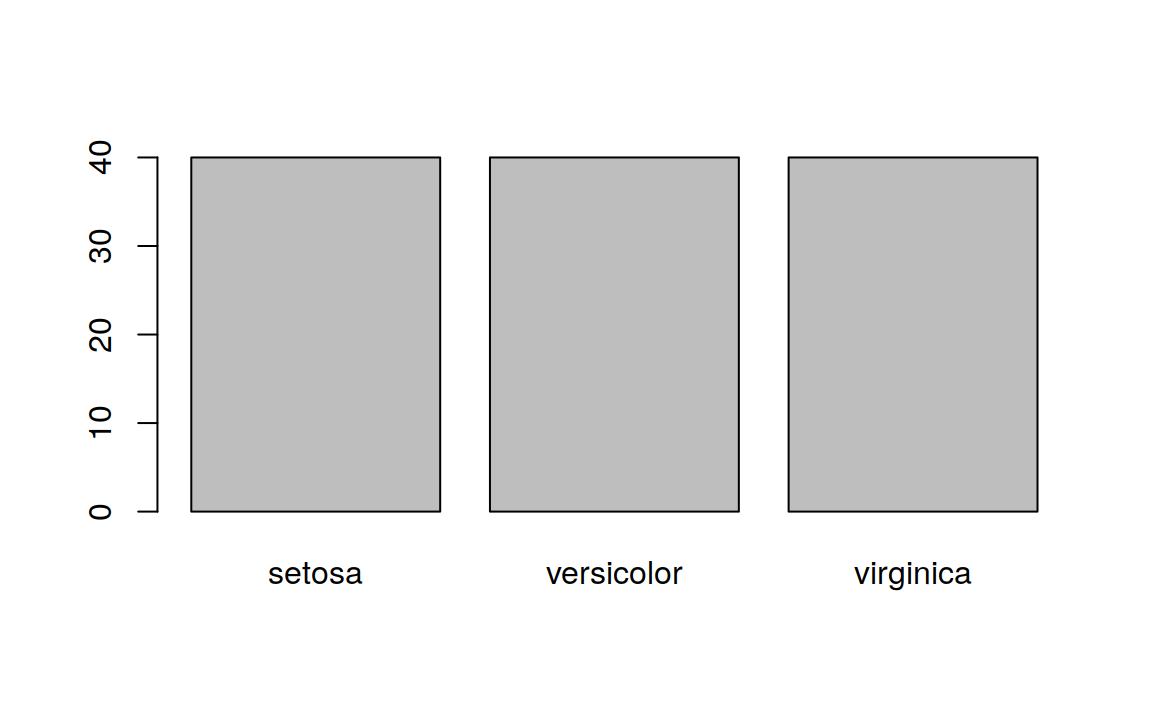
\includegraphics[width=0.7\linewidth]{regression_902-fitting_neural_network_files/figure-latex/unnamed-chunk-12-1} \end{center}

\hypertarget{a-fast-cross-validation}{%
\section{A (fast) cross validation}\label{a-fast-cross-validation}}

Cross validation is another very important step of building predictive models. While there are different kind of cross validation methods, the basic idea is repeating the following process a number of time:

\textbf{train-test split}

\begin{itemize}
\tightlist
\item
  Do the train-test split
\item
  Fit the model to the train set
\item
  Test the model on the test set
\item
  Calculate the prediction error
\item
  Repeat the process K times
\end{itemize}

Then by calculating the average error we can get a grasp of how the model is doing.

We are going to implement a fast cross validation using a for loop for the neural network and the cv.glm() function in the boot package for the linear model.
As far as I know, there is no built-in function in R to perform cross-validation on this kind of neural network, if you do know such a function, please let me know in the comments. Here is the 10 fold cross-validated MSE for the linear model:

\begin{Shaded}
\begin{Highlighting}[]
\KeywordTok{library}\NormalTok{(boot)}
\KeywordTok{set.seed}\NormalTok{(}\DecValTok{200}\NormalTok{)}
\NormalTok{lm.fit <-}\StringTok{ }\KeywordTok{glm}\NormalTok{(medv}\OperatorTok{~}\NormalTok{.,}\DataTypeTok{data=}\NormalTok{data)}
\KeywordTok{cv.glm}\NormalTok{(data,lm.fit,}\DataTypeTok{K=}\DecValTok{10}\NormalTok{)}\OperatorTok{$}\NormalTok{delta[}\DecValTok{1}\NormalTok{]}
\CommentTok{#> [1] 23.2}
\end{Highlighting}
\end{Shaded}

Now the net. Note that I am splitting the data in this way: 90\% train set and 10\% test set in a random way for 10 times. I am also initializing a progress bar using the plyr library because I want to keep an eye on the status of the process since the fitting of the neural network may take a while.

\begin{Shaded}
\begin{Highlighting}[]
\KeywordTok{set.seed}\NormalTok{(}\DecValTok{450}\NormalTok{)}
\NormalTok{cv.error <-}\StringTok{ }\OtherTok{NULL}
\NormalTok{k <-}\StringTok{ }\DecValTok{10}

\KeywordTok{library}\NormalTok{(plyr) }
\NormalTok{pbar <-}\StringTok{ }\KeywordTok{create_progress_bar}\NormalTok{(}\StringTok{'text'}\NormalTok{)}
\NormalTok{pbar}\OperatorTok{$}\KeywordTok{init}\NormalTok{(k)}
\CommentTok{#> }
  \OperatorTok{|}\StringTok{                                                                       }
\StringTok{  }\ErrorTok{|}\StringTok{                                                                 }\ErrorTok{|}\StringTok{   }\DecValTok{0}\NormalTok{%}

\ControlFlowTok{for}\NormalTok{(i }\ControlFlowTok{in} \DecValTok{1}\OperatorTok{:}\NormalTok{k)\{}
\NormalTok{    index <-}\StringTok{ }\KeywordTok{sample}\NormalTok{(}\DecValTok{1}\OperatorTok{:}\KeywordTok{nrow}\NormalTok{(data),}\KeywordTok{round}\NormalTok{(}\FloatTok{0.9}\OperatorTok{*}\KeywordTok{nrow}\NormalTok{(data)))}
\NormalTok{    train.cv <-}\StringTok{ }\NormalTok{scaled[index,]}
\NormalTok{    test.cv <-}\StringTok{ }\NormalTok{scaled[}\OperatorTok{-}\NormalTok{index,]}
    
\NormalTok{    nn <-}\StringTok{ }\KeywordTok{neuralnet}\NormalTok{(f,}\DataTypeTok{data=}\NormalTok{train.cv,}\DataTypeTok{hidden=}\KeywordTok{c}\NormalTok{(}\DecValTok{5}\NormalTok{,}\DecValTok{2}\NormalTok{),}\DataTypeTok{linear.output=}\NormalTok{T)}
    
\NormalTok{    pr.nn <-}\StringTok{ }\KeywordTok{compute}\NormalTok{(nn,test.cv[,}\DecValTok{1}\OperatorTok{:}\DecValTok{13}\NormalTok{])}
\NormalTok{    pr.nn <-}\StringTok{ }\NormalTok{pr.nn}\OperatorTok{$}\NormalTok{net.result}\OperatorTok{*}\NormalTok{(}\KeywordTok{max}\NormalTok{(data}\OperatorTok{$}\NormalTok{medv)}\OperatorTok{-}\KeywordTok{min}\NormalTok{(data}\OperatorTok{$}\NormalTok{medv))}\OperatorTok{+}\KeywordTok{min}\NormalTok{(data}\OperatorTok{$}\NormalTok{medv)}
    
\NormalTok{    test.cv.r <-}\StringTok{ }\NormalTok{(test.cv}\OperatorTok{$}\NormalTok{medv)}\OperatorTok{*}\NormalTok{(}\KeywordTok{max}\NormalTok{(data}\OperatorTok{$}\NormalTok{medv)}\OperatorTok{-}\KeywordTok{min}\NormalTok{(data}\OperatorTok{$}\NormalTok{medv))}\OperatorTok{+}\KeywordTok{min}\NormalTok{(data}\OperatorTok{$}\NormalTok{medv)}
    
\NormalTok{    cv.error[i] <-}\StringTok{ }\KeywordTok{sum}\NormalTok{((test.cv.r }\OperatorTok{-}\StringTok{ }\NormalTok{pr.nn)}\OperatorTok{^}\DecValTok{2}\NormalTok{)}\OperatorTok{/}\KeywordTok{nrow}\NormalTok{(test.cv)}
    
\NormalTok{    pbar}\OperatorTok{$}\KeywordTok{step}\NormalTok{()}
\NormalTok{\}}
\CommentTok{#> }
  \OperatorTok{|}\StringTok{                                                                       }
\StringTok{  }\ErrorTok{|======}\StringTok{                                                           }\ErrorTok{|}\StringTok{  }\DecValTok{10}\NormalTok
  \OperatorTok{|}\StringTok{                                                                       }
\StringTok{  }\ErrorTok{|====================}\StringTok{                                             }\ErrorTok{|}\StringTok{  }\DecValTok{30}\NormalTok
  \OperatorTok{|}\StringTok{                                                                       }
\StringTok{  }\ErrorTok{|================================}\StringTok{                                 }\ErrorTok{|}\StringTok{  }\DecValTok{50}\NormalTok
  \OperatorTok{|}\StringTok{                                                                       }
\StringTok{  }\ErrorTok{|==============================================}\StringTok{                   }\ErrorTok{|}\StringTok{  }\DecValTok{70}\NormalTok
  \OperatorTok{|}\StringTok{                                                                       }
\StringTok{  }\ErrorTok{|==========================================================}\StringTok{       }\ErrorTok{|}\StringTok{  }\DecValTok{90}\NormalTok
\end{Highlighting}
\end{Shaded}

After a while, the process is done, we calculate the average MSE and plot the results as a boxplot

\begin{Shaded}
\begin{Highlighting}[]
\KeywordTok{mean}\NormalTok{(cv.error)}
\CommentTok{#> [1] 7.64}
\end{Highlighting}
\end{Shaded}

\begin{Shaded}
\begin{Highlighting}[]
\NormalTok{cv.error}
\CommentTok{#>  [1] 13.33  7.10  6.58  5.70  6.84  5.77 10.75  5.38  9.45  5.50}
\end{Highlighting}
\end{Shaded}

The code for the box plot:
The code above outputs the following boxplot:

\begin{Shaded}
\begin{Highlighting}[]
\KeywordTok{boxplot}\NormalTok{(cv.error,}\DataTypeTok{xlab=}\StringTok{'MSE CV'}\NormalTok{,}\DataTypeTok{col=}\StringTok{'cyan'}\NormalTok{,}
        \DataTypeTok{border=}\StringTok{'blue'}\NormalTok{,}\DataTypeTok{names=}\StringTok{'CV error (MSE)'}\NormalTok{,}
        \DataTypeTok{main=}\StringTok{'CV error (MSE) for NN'}\NormalTok{,}\DataTypeTok{horizontal=}\OtherTok{TRUE}\NormalTok{)}
\end{Highlighting}
\end{Shaded}

\begin{center}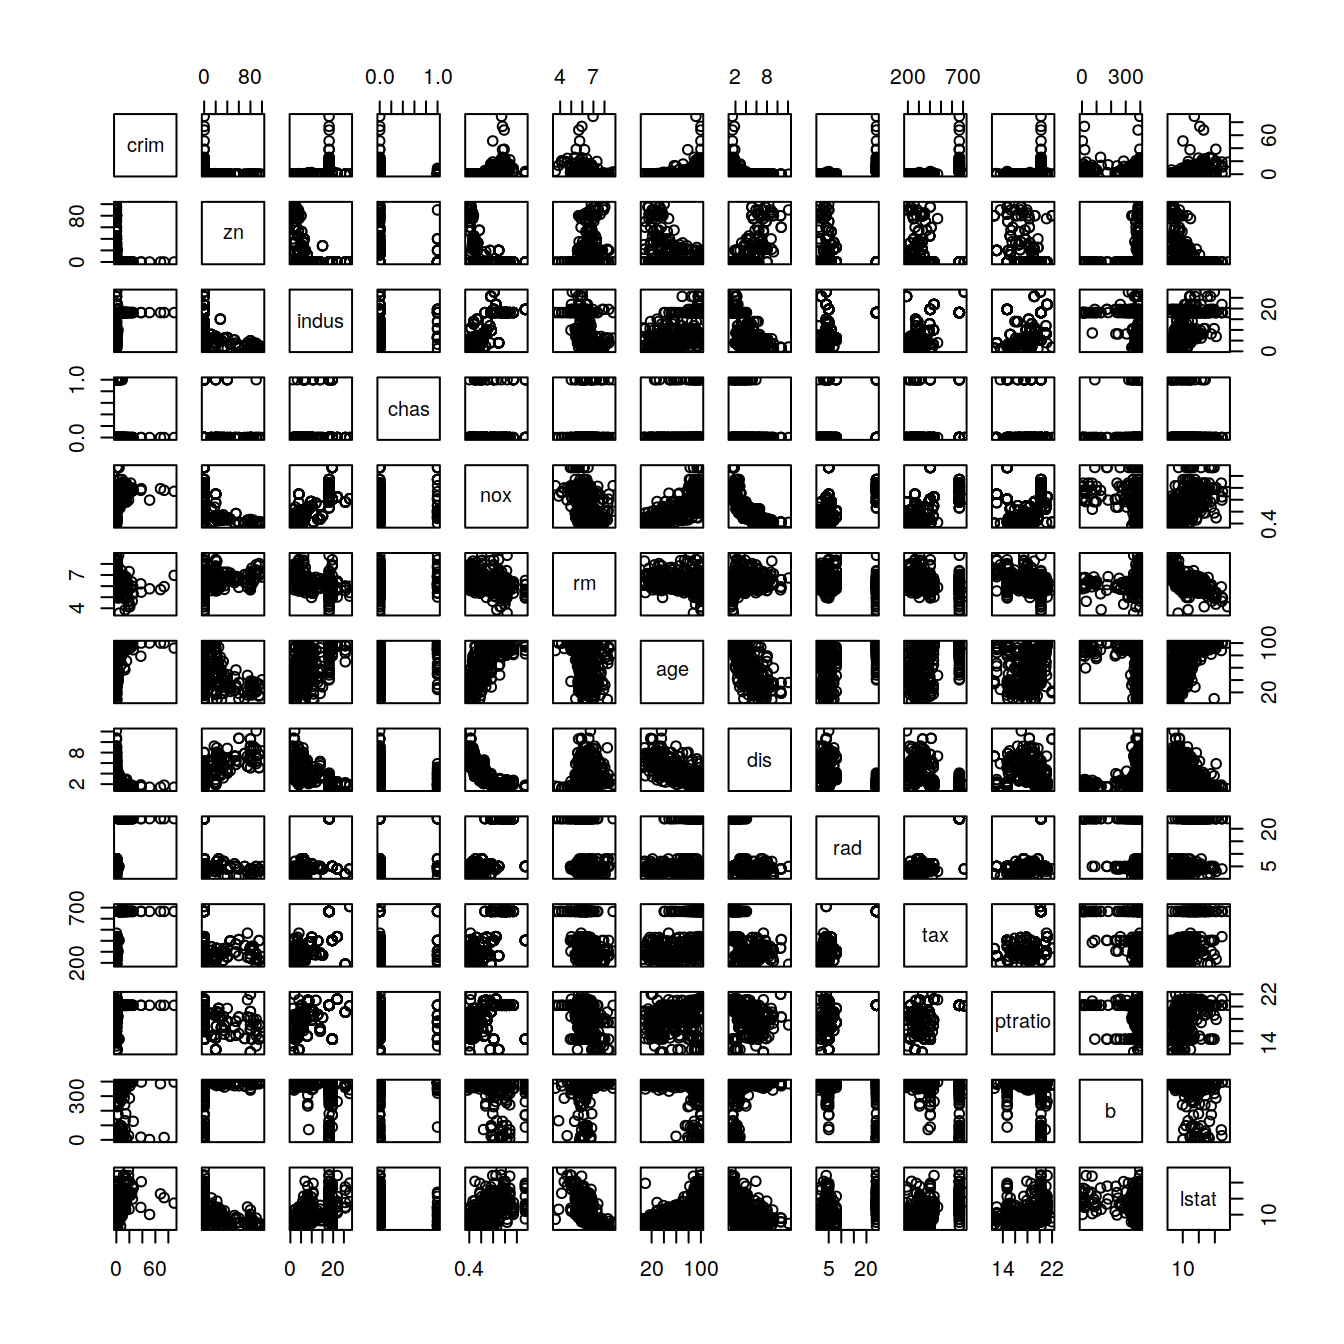
\includegraphics[width=0.7\linewidth]{regression_902-fitting_neural_network_files/figure-latex/unnamed-chunk-17-1} \end{center}

As you can see, the average MSE for the neural network (10.33) is lower than the one of the linear model although there seems to be a certain degree of variation in the MSEs of the cross validation. This may depend on the splitting of the data or the random initialization of the weights in the net. By running the simulation different times with different seeds you can get a more precise point estimate for the average MSE.

\hypertarget{a-final-note-on-model-interpretability}{%
\section{A final note on model interpretability}\label{a-final-note-on-model-interpretability}}

Neural networks resemble black boxes a lot: explaining their outcome is much more difficult than explaining the outcome of simpler model such as a linear model. Therefore, depending on the kind of application you need, you might want to take into account this factor too. Furthermore, as you have seen above, extra care is needed to fit a neural network and small changes can lead to different results.

A gist with the full code for this post can be found here.

Thank you for reading this post, leave a comment below if you have any question.

\hypertarget{visualization-of-neural-networks}{%
\chapter{Visualization of neural networks}\label{visualization-of-neural-networks}}

\url{https://beckmw.wordpress.com/tag/neuralnet/}

In my last post I said I wasn't going to write anymore about neural networks (i.e., multilayer feedforward perceptron, supervised ANN, etc.). That was a lie. I've received several requests to update the neural network plotting function described in the original post. As previously explained, R does not provide a lot of options for visualizing neural networks. The only option I know of is a plotting method for objects from the neuralnet package. This may be my opinion, but I think this plot leaves much to be desired (see below). Also, no plotting methods exist for neural networks created in other packages, i.e., nnet and RSNNS. These packages are the only ones listed on the CRAN task view, so I've updated my original plotting function to work with all three. Additionally, I've added a new option for plotting a raw weight vector to allow use with neural networks created elsewhere. This blog describes these changes, as well as some new arguments added to the original function.

As usual, I'll simulate some data to use for creating the neural networks. The dataset contains eight input variables and two output variables. The final dataset is a data frame with all variables, as well as separate data frames for the input and output variables. I've retained separate datasets based on the syntax for each package.

\begin{Shaded}
\begin{Highlighting}[]
\KeywordTok{library}\NormalTok{(clusterGeneration)}
\CommentTok{#> Loading required package: MASS}
\KeywordTok{library}\NormalTok{(tictoc)}
 
\NormalTok{seed.val<-}\StringTok{ }\DecValTok{12345}
\KeywordTok{set.seed}\NormalTok{(seed.val)}
 
\NormalTok{num.vars<-}\DecValTok{8}
\NormalTok{num.obs<-}\DecValTok{1000}
 
\CommentTok{# input variables}
\NormalTok{cov.mat <-}\KeywordTok{genPositiveDefMat}\NormalTok{(num.vars,}\DataTypeTok{covMethod=}\KeywordTok{c}\NormalTok{(}\StringTok{"unifcorrmat"}\NormalTok{))}\OperatorTok{$}\NormalTok{Sigma}
\NormalTok{rand.vars <-}\KeywordTok{mvrnorm}\NormalTok{(num.obs,}\KeywordTok{rep}\NormalTok{(}\DecValTok{0}\NormalTok{,num.vars),}\DataTypeTok{Sigma=}\NormalTok{cov.mat)}
 
\CommentTok{# output variables}
\NormalTok{parms <-}\KeywordTok{runif}\NormalTok{(num.vars,}\OperatorTok{-}\DecValTok{10}\NormalTok{,}\DecValTok{10}\NormalTok{)}
\NormalTok{y1 <-}\StringTok{ }\NormalTok{rand.vars }\OperatorTok\StringTok{ }\KeywordTok{matrix}\NormalTok{(parms) }\OperatorTok{+}\StringTok{ }\KeywordTok{rnorm}\NormalTok{(num.obs,}\DataTypeTok{sd=}\DecValTok{20}\NormalTok{)}
\NormalTok{parms2 <-}\StringTok{ }\KeywordTok{runif}\NormalTok{(num.vars,}\OperatorTok{-}\DecValTok{10}\NormalTok{,}\DecValTok{10}\NormalTok{)}
\NormalTok{y2 <-}\StringTok{ }\NormalTok{rand.vars }\OperatorTok\StringTok{ }\KeywordTok{matrix}\NormalTok{(parms2) }\OperatorTok{+}\StringTok{ }\KeywordTok{rnorm}\NormalTok{(num.obs,}\DataTypeTok{sd=}\DecValTok{20}\NormalTok{)}
 
\CommentTok{# final datasets}
\NormalTok{rand.vars <-}\StringTok{ }\KeywordTok{data.frame}\NormalTok{(rand.vars)}
\NormalTok{resp <-}\StringTok{ }\KeywordTok{data.frame}\NormalTok{(y1,y2)}
\KeywordTok{names}\NormalTok{(resp) <-}\StringTok{ }\KeywordTok{c}\NormalTok{(}\StringTok{'Y1'}\NormalTok{,}\StringTok{'Y2'}\NormalTok{)}
\NormalTok{dat.in <-}\StringTok{ }\KeywordTok{data.frame}\NormalTok{(resp, rand.vars)}
\end{Highlighting}
\end{Shaded}

\begin{Shaded}
\begin{Highlighting}[]
\NormalTok{dplyr}\OperatorTok{::}\KeywordTok{glimpse}\NormalTok{(dat.in)}
\CommentTok{#> Observations: 1,000}
\CommentTok{#> Variables: 10}
\CommentTok{#> $ Y1 <dbl> 25.442, -14.578, -36.214, 15.216, -6.393, -20.849, -28.665,...}
\CommentTok{#> $ Y2 <dbl> 16.9, 38.8, 31.2, -31.2, 93.3, 11.7, 59.7, -103.5, -49.8, 5...}
\CommentTok{#> $ X1 <dbl> 3.138, -0.705, -4.373, 0.837, 0.787, 1.923, -1.419, 1.121, ...}
\CommentTok{#> $ X2 <dbl> 0.195, -0.302, 0.773, 1.311, 3.506, 1.245, 3.800, -0.165, 0...}
\CommentTok{#> $ X3 <dbl> -1.795, -2.596, 2.308, 4.081, -3.921, 1.473, -0.926, 7.101,...}
\CommentTok{#> $ X4 <dbl> -2.7216, 3.0589, 1.2455, 3.4607, 2.3775, -2.9833, 2.6669, -...}
\CommentTok{#> $ X5 <dbl> 0.0407, 0.7602, -3.0217, -4.2799, 2.0859, 1.4765, 0.0561, 2...}
\CommentTok{#> $ X6 <dbl> -1.4820, -0.5014, 0.0603, -1.8551, 2.2817, 1.7386, 1.7450, ...}
\CommentTok{#> $ X7 <dbl> -0.7169, -0.3618, -1.5283, 4.2026, -6.1548, -0.3545, -6.028...}
\CommentTok{#> $ X8 <dbl> 1.152, 1.810, -1.357, 0.598, -1.425, -1.210, -1.004, 2.494,...}
\end{Highlighting}
\end{Shaded}

The various neural network packages are used to create separate models for plotting.

\begin{Shaded}
\begin{Highlighting}[]
\CommentTok{# first model with nnet}
\CommentTok{#nnet function from nnet package}
\KeywordTok{library}\NormalTok{(nnet)}
\KeywordTok{set.seed}\NormalTok{(seed.val)}
\KeywordTok{tic}\NormalTok{()}
\NormalTok{mod1 <-}\StringTok{ }\KeywordTok{nnet}\NormalTok{(rand.vars, resp, }\DataTypeTok{data =}\NormalTok{ dat.in, }\DataTypeTok{size =} \DecValTok{10}\NormalTok{, }\DataTypeTok{linout =}\NormalTok{ T)}
\CommentTok{#> # weights:  112}
\CommentTok{#> initial  value 4784162.893260 }
\CommentTok{#> iter  10 value 1794537.980652}
\CommentTok{#> iter  20 value 1577753.498759}
\CommentTok{#> iter  30 value 1485254.945755}
\CommentTok{#> iter  40 value 1449238.248788}
\CommentTok{#> iter  50 value 1427720.291804}
\CommentTok{#> iter  60 value 1416977.236373}
\CommentTok{#> iter  70 value 1405167.753521}
\CommentTok{#> iter  80 value 1395046.792257}
\CommentTok{#> iter  90 value 1370522.267277}
\CommentTok{#> iter 100 value 1363709.540981}
\CommentTok{#> final  value 1363709.540981 }
\CommentTok{#> stopped after 100 iterations}
\KeywordTok{toc}\NormalTok{()}
\CommentTok{#> 0.195 sec elapsed}
\end{Highlighting}
\end{Shaded}

\begin{Shaded}
\begin{Highlighting}[]
\CommentTok{# nn <- neuralnet(form.in,}
\CommentTok{#                 data = dat.sc,}
\CommentTok{#                 # hidden = c(13, 10, 3),}
\CommentTok{#                 hidden = c(5),}
\CommentTok{#                 act.fct = "tanh",}
\CommentTok{#                 linear.output = FALSE,}
\CommentTok{#                 lifesign = "minimal")}
\end{Highlighting}
\end{Shaded}

\begin{Shaded}
\begin{Highlighting}[]
\CommentTok{# 2nd model with neuralnet}
\CommentTok{# neuralnet function from neuralnet package, notice use of only one response}
\KeywordTok{library}\NormalTok{(neuralnet)}

\NormalTok{softplus <-}\StringTok{ }\ControlFlowTok{function}\NormalTok{(x) }\KeywordTok{log}\NormalTok{(}\DecValTok{1} \OperatorTok{+}\StringTok{ }\KeywordTok{exp}\NormalTok{(x))}
\NormalTok{sigmoid  <-}\StringTok{ }\ControlFlowTok{function}\NormalTok{(x) }\KeywordTok{log}\NormalTok{(}\DecValTok{1} \OperatorTok{+}\StringTok{ }\KeywordTok{exp}\NormalTok{(}\OperatorTok{-}\NormalTok{x))}

\NormalTok{dat.sc <-}\StringTok{ }\KeywordTok{scale}\NormalTok{(dat.in)}
\NormalTok{form.in <-}\StringTok{ }\KeywordTok{as.formula}\NormalTok{(}\StringTok{'Y1 ~ X1+X2+X3+X4+X5+X6+X7+X8'}\NormalTok{)}
\KeywordTok{set.seed}\NormalTok{(seed.val)}
\KeywordTok{tic}\NormalTok{()}
\NormalTok{mod2 <-}\StringTok{ }\KeywordTok{neuralnet}\NormalTok{(form.in, }\DataTypeTok{data =}\NormalTok{ dat.sc, }\DataTypeTok{hidden =} \DecValTok{10}\NormalTok{, }\DataTypeTok{lifesign =} \StringTok{"minimal"}\NormalTok{,}
                  \DataTypeTok{linear.output =} \OtherTok{FALSE}\NormalTok{,}
                  \DataTypeTok{act.fct =} \StringTok{"tanh"}\NormalTok{)}
\CommentTok{#> hidden: 10    thresh: 0.01    rep: 1/1    steps:   26361 error: 160.06372    time: 58.25 secs}
\KeywordTok{toc}\NormalTok{()}
\CommentTok{#> 58.265 sec elapsed}
\end{Highlighting}
\end{Shaded}

\begin{Shaded}
\begin{Highlighting}[]
\CommentTok{# third model with RSNNS}
\CommentTok{# mlp function from RSNNS package}
\KeywordTok{library}\NormalTok{(RSNNS)}
\CommentTok{#> Loading required package: Rcpp}
\KeywordTok{set.seed}\NormalTok{(seed.val)}
\KeywordTok{tic}\NormalTok{()}
\NormalTok{mod3 <-}\StringTok{ }\KeywordTok{mlp}\NormalTok{(rand.vars, resp, }\DataTypeTok{size =} \DecValTok{10}\NormalTok{, }\DataTypeTok{linOut =}\NormalTok{ T)}
\KeywordTok{toc}\NormalTok{()}
\CommentTok{#> 0.406 sec elapsed}
\end{Highlighting}
\end{Shaded}

I've noticed some differences between the functions that could lead to some confusion. For simplicity, the above code represents my interpretation of the most direct way to create a neural network in each package. Be very aware that direct comparison of results is not advised given that the default arguments differ between the packages. A few key differences are as follows, although many others should be noted. First, the functions differ in the methods for passing the primary input variables.

The \texttt{nnet} function can take separate (or combined) x and y inputs as data frames or as a formula, the \texttt{neuralnet} function can only use a formula as input, and the mlp function can only take a data frame as combined or separate variables as input. As far as I know, the neuralnet function is not capable of modelling multiple response variables, unless the response is a categorical variable that uses one node for each outcome. Additionally, the default output for the neuralnet function is linear, whereas the opposite is true for the other two functions.

Specifics aside, here's how to use the updated plot function. Note that the same syntax is used to plot each model

\begin{Shaded}
\begin{Highlighting}[]
\CommentTok{# import the function from Github}
\KeywordTok{library}\NormalTok{(devtools)}
\KeywordTok{source_url}\NormalTok{(}\StringTok{'https://gist.githubusercontent.com/fawda123/7471137/raw/466c1474d0a505ff044412703516c34f1a4684a5/nnet_plot_update.r'}\NormalTok{)}
\CommentTok{#> SHA-1 hash of file is 74c80bd5ddbc17ab3ae5ece9c0ed9beb612e87ef}
 
\CommentTok{# plot each model}
\KeywordTok{plot.nnet}\NormalTok{(mod1)}
\CommentTok{#> Loading required package: scales}
\CommentTok{#> Loading required package: reshape}
\KeywordTok{plot.nnet}\NormalTok{(mod2) }
\KeywordTok{plot.nnet}\NormalTok{(mod3)}
\CommentTok{#> Warning in plot.nnet(mod3): Bias layer not applicable for rsnns object}
\end{Highlighting}
\end{Shaded}

\begin{center}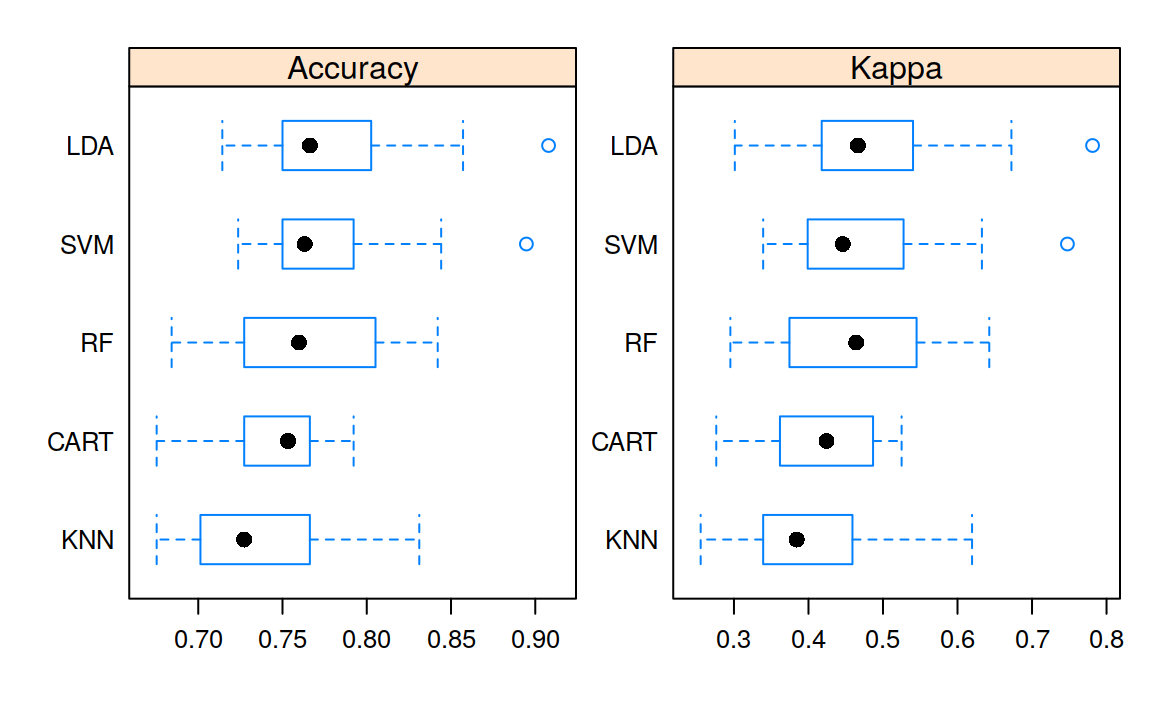
\includegraphics[width=0.7\linewidth]{regression_903-visualization_nn_files/figure-latex/unnamed-chunk-5-1} 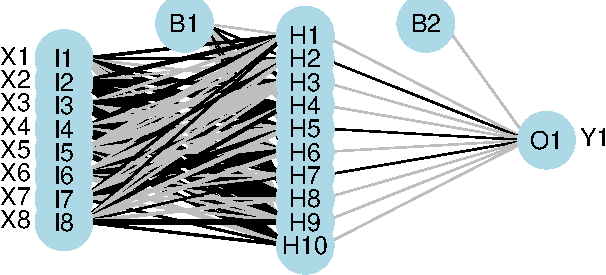
\includegraphics[width=0.7\linewidth]{regression_903-visualization_nn_files/figure-latex/unnamed-chunk-5-2} 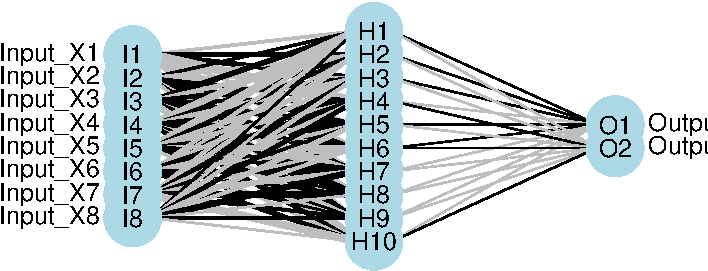
\includegraphics[width=0.7\linewidth]{regression_903-visualization_nn_files/figure-latex/unnamed-chunk-5-3} \end{center}

The plotting function can also now be used with an arbitrary weight vector, rather than a specific model object. The struct argument must also be included if this option is used. I thought the easiest way to use the plotting function with your own weights was to have the input weights as a numeric vector, including bias layers. I've shown how this can be done using the weights directly from mod1 for simplicity.

\begin{Shaded}
\begin{Highlighting}[]
\NormalTok{wts.in <-}\StringTok{ }\NormalTok{mod1}\OperatorTok{$}\NormalTok{wts}
\NormalTok{struct <-}\StringTok{ }\NormalTok{mod1}\OperatorTok{$}\NormalTok{n}
\KeywordTok{plot.nnet}\NormalTok{(wts.in,}\DataTypeTok{struct=}\NormalTok{struct)}
\end{Highlighting}
\end{Shaded}

\begin{center}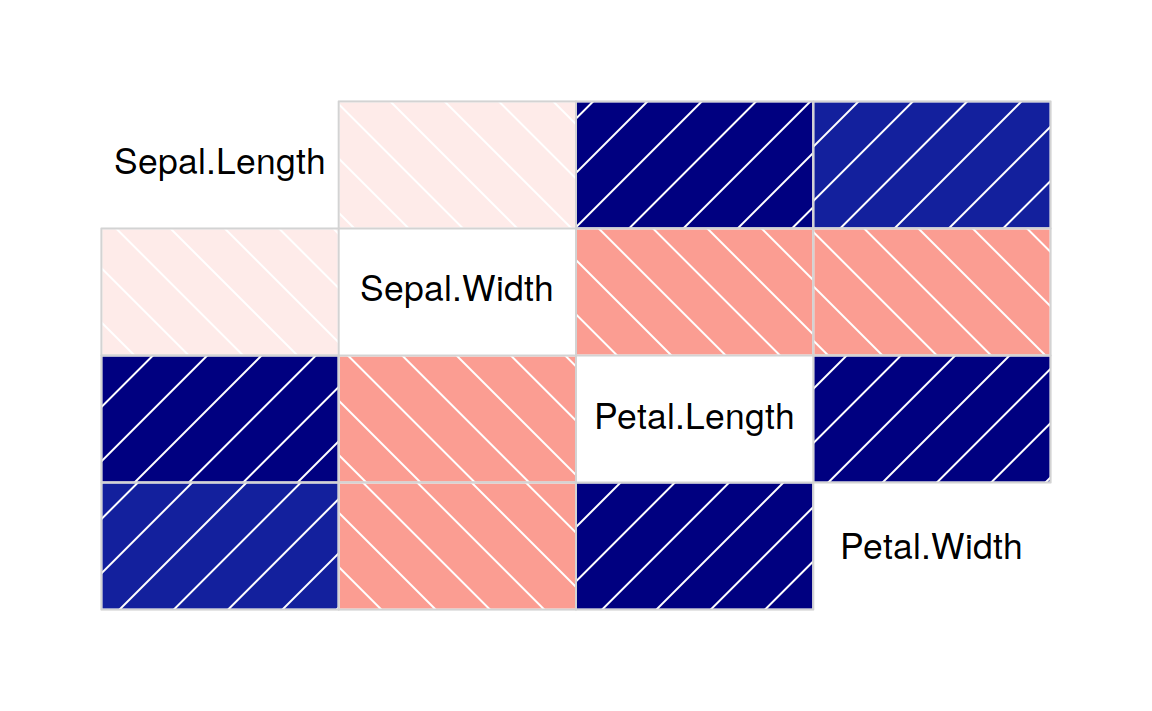
\includegraphics[width=0.7\linewidth]{regression_903-visualization_nn_files/figure-latex/unnamed-chunk-6-1} \end{center}

Note that \texttt{wts.in} is a numeric vector with length equal to the expected given the architecture (i.e., for 8 10 2 network, 100 connection weights plus 12 bias weights). The plot should look the same as the plot for the neural network from nnet.

The weights in the input vector need to be in a specific order for correct plotting. I realize this is not clear by looking directly at wt.in but this was the simplest approach I could think of. The weight vector shows the weights for each hidden node in sequence, starting with the bias input for each node, then the weights for each output node in sequence, starting with the bias input for each output node. Note that the bias layer has to be included even if the network was not created with biases. If this is the case, simply input a random number where the bias values should go and use the argument bias=F. I'll show the correct order of the weights using an example with plot.nn from the neuralnet package since the weights are included directly on the plot.

If we pretend that the above figure wasn't created in R, we would input the mod.in argument for the updated plotting function as follows. Also note that struct must be included if using this approach.

\begin{Shaded}
\begin{Highlighting}[]
\NormalTok{mod.in<-}\KeywordTok{c}\NormalTok{(}\FloatTok{13.12}\NormalTok{,}\FloatTok{1.49}\NormalTok{,}\FloatTok{0.16}\NormalTok{,}\OperatorTok{-}\FloatTok{0.11}\NormalTok{,}\OperatorTok{-}\FloatTok{0.19}\NormalTok{,}\OperatorTok{-}\FloatTok{0.16}\NormalTok{,}\FloatTok{0.56}\NormalTok{,}\OperatorTok{-}\FloatTok{0.52}\NormalTok{,}\FloatTok{0.81}\NormalTok{)}
\NormalTok{struct<-}\KeywordTok{c}\NormalTok{(}\DecValTok{2}\NormalTok{,}\DecValTok{2}\NormalTok{,}\DecValTok{1}\NormalTok{) }\CommentTok{#two inputs, two hidden, one output }
\KeywordTok{plot.nnet}\NormalTok{(mod.in, }\DataTypeTok{struct=}\NormalTok{struct)}
\end{Highlighting}
\end{Shaded}

\begin{center}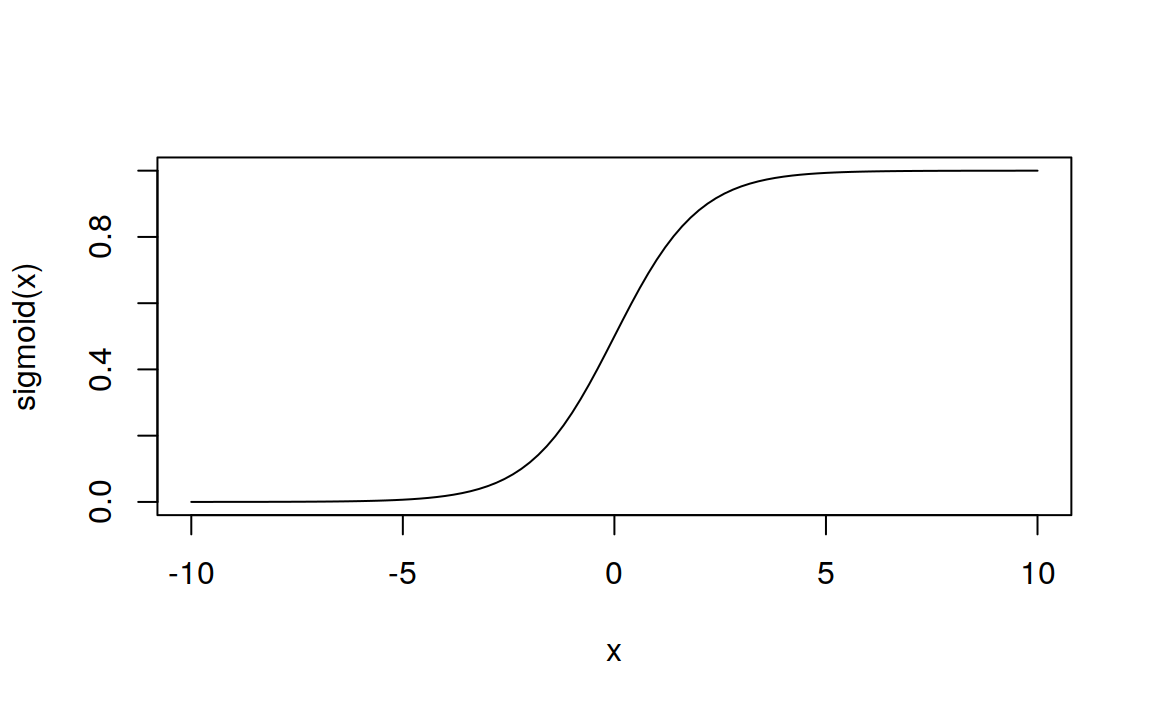
\includegraphics[width=0.7\linewidth]{regression_903-visualization_nn_files/figure-latex/unnamed-chunk-7-1} \end{center}

Note the comparability with the figure created using the neuralnet package. That is, larger weights have thicker lines and color indicates sign (+ black, -- grey).

One of these days I'll actually put these functions in a package. In the meantime, please let me know if any bugs are encountered.

\hypertarget{caret-and-plot-nn}{%
\section{caret and plot NN}\label{caret-and-plot-nn}}

I've changed the function to work with neural networks created using the train function from the caret package. The link above is updated but you can also grab it here.

\begin{Shaded}
\begin{Highlighting}[]
\KeywordTok{library}\NormalTok{(caret)}
\CommentTok{#> Loading required package: lattice}
\CommentTok{#> Loading required package: ggplot2}
\CommentTok{#> Registered S3 methods overwritten by 'ggplot2':}
\CommentTok{#>   method         from }
\CommentTok{#>   [.quosures     rlang}
\CommentTok{#>   c.quosures     rlang}
\CommentTok{#>   print.quosures rlang}
\CommentTok{#> }
\CommentTok{#> Attaching package: 'caret'}
\CommentTok{#> The following objects are masked from 'package:RSNNS':}
\CommentTok{#> }
\CommentTok{#>     confusionMatrix, train}
\NormalTok{mod4 <-}\StringTok{ }\KeywordTok{train}\NormalTok{(Y1 }\OperatorTok{~}\NormalTok{., }\DataTypeTok{method=}\StringTok{'nnet'}\NormalTok{, }\DataTypeTok{data=}\NormalTok{dat.in, }\DataTypeTok{linout=}\NormalTok{T)}
\end{Highlighting}
\end{Shaded}

\begin{Shaded}
\begin{Highlighting}[]
\KeywordTok{plot.nnet}\NormalTok{(mod4,}\DataTypeTok{nid=}\NormalTok{T)}
\CommentTok{#> Warning in plot.nnet(mod4, nid = T): Using best nnet model from train}
\CommentTok{#> output}
\end{Highlighting}
\end{Shaded}

\begin{center}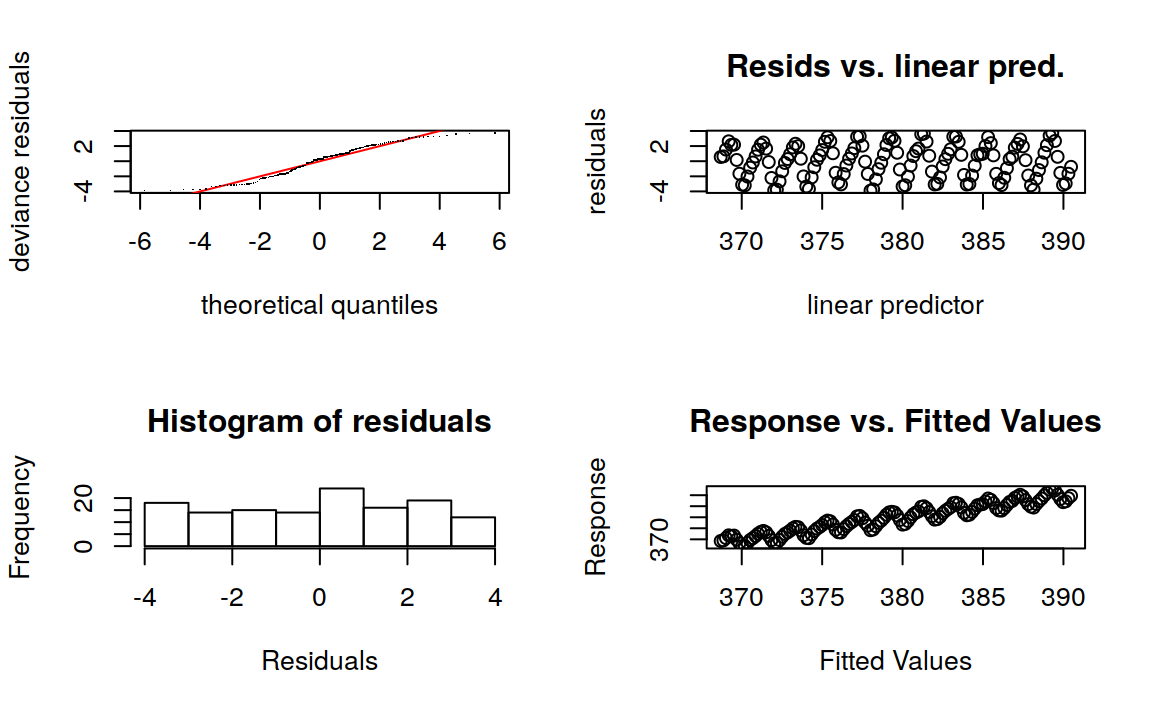
\includegraphics[width=0.7\linewidth]{regression_903-visualization_nn_files/figure-latex/unnamed-chunk-8-1} \end{center}

\begin{Shaded}
\begin{Highlighting}[]
\NormalTok{fact<-}\KeywordTok{factor}\NormalTok{(}\KeywordTok{sample}\NormalTok{(}\KeywordTok{c}\NormalTok{(}\StringTok{'a'}\NormalTok{,}\StringTok{'b'}\NormalTok{,}\StringTok{'c'}\NormalTok{),}\DataTypeTok{size=}\NormalTok{num.obs,}\DataTypeTok{replace=}\NormalTok{T))}
\NormalTok{form.in<-}\KeywordTok{formula}\NormalTok{(}\StringTok{'cbind(Y2,Y1)~X1+X2+X3+fact'}\NormalTok{)}
\NormalTok{mod5<-}\KeywordTok{nnet}\NormalTok{(form.in,}\DataTypeTok{data=}\KeywordTok{cbind}\NormalTok{(dat.in,fact),}\DataTypeTok{size=}\DecValTok{10}\NormalTok{,}\DataTypeTok{linout=}\NormalTok{T)}
\CommentTok{#> # weights:  82}
\CommentTok{#> initial  value 4799569.423556 }
\CommentTok{#> iter  10 value 2864553.218126}
\CommentTok{#> iter  20 value 2595828.194160}
\CommentTok{#> iter  30 value 2517965.483941}
\CommentTok{#> iter  40 value 2464882.178217}
\CommentTok{#> iter  50 value 2444238.700834}
\CommentTok{#> iter  60 value 2424302.290643}
\CommentTok{#> iter  70 value 2395226.949866}
\CommentTok{#> iter  80 value 2375558.751266}
\CommentTok{#> iter  90 value 2343011.050867}
\CommentTok{#> iter 100 value 2298860.593948}
\CommentTok{#> final  value 2298860.593948 }
\CommentTok{#> stopped after 100 iterations}
\KeywordTok{plot.nnet}\NormalTok{(mod5,}\DataTypeTok{nid=}\NormalTok{T)}
\end{Highlighting}
\end{Shaded}

\begin{center}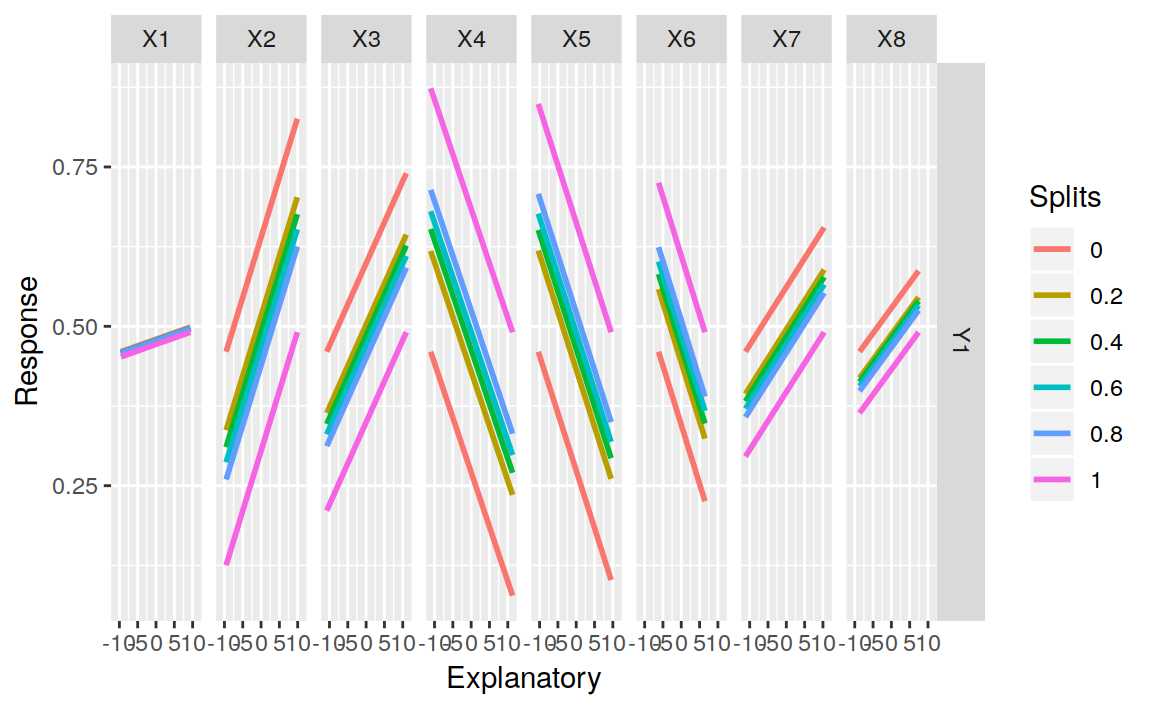
\includegraphics[width=0.7\linewidth]{regression_903-visualization_nn_files/figure-latex/unnamed-chunk-9-1} \end{center}

\hypertarget{multiple-hidden-layers}{%
\section{Multiple hidden layers}\label{multiple-hidden-layers}}

More updates\ldots{} I've now modified the function to plot multiple hidden layers for networks created using the mlp function in the \texttt{RSNNS} package and neuralnet in the neuralnet package. As far as I know, these are the only neural network functions in R that can create multiple hidden layers. All others use a single hidden layer. I have not tested the plotting function using manual input for the weight vectors with multiple hidden layers. My guess is it won't work but I can't be bothered to change the function unless it's specifically requested. The updated function can be grabbed here (all above links to the function have also been changed).

\begin{Shaded}
\begin{Highlighting}[]
\KeywordTok{library}\NormalTok{(RSNNS)}
 
\CommentTok{# neural net with three hidden layers, 9, 11, and 8 nodes in each}
\KeywordTok{tic}\NormalTok{()}
\NormalTok{mod <-}\KeywordTok{mlp}\NormalTok{(rand.vars, resp, }
          \DataTypeTok{size =} \KeywordTok{c}\NormalTok{(}\DecValTok{9}\NormalTok{,}\DecValTok{11}\NormalTok{,}\DecValTok{8}\NormalTok{), }
          \DataTypeTok{linOut =}\NormalTok{ T)}
\KeywordTok{toc}\NormalTok{()}
\CommentTok{#> 0.425 sec elapsed}
\KeywordTok{par}\NormalTok{(}\DataTypeTok{mar=}\KeywordTok{numeric}\NormalTok{(}\DecValTok{4}\NormalTok{),}\DataTypeTok{family=}\StringTok{'serif'}\NormalTok{)}
\KeywordTok{plot.nnet}\NormalTok{(mod)}
\CommentTok{#> Warning in plot.nnet(mod): Bias layer not applicable for rsnns object}
\end{Highlighting}
\end{Shaded}

\begin{center}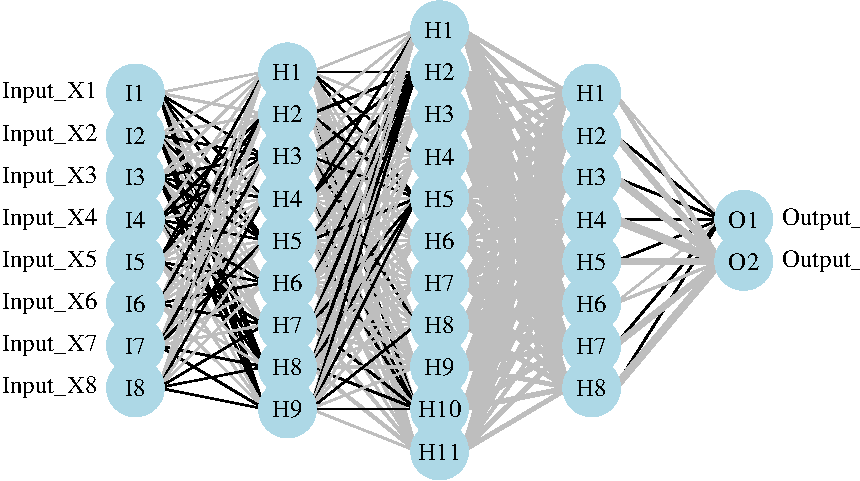
\includegraphics[width=0.7\linewidth]{regression_903-visualization_nn_files/figure-latex/run-rsnns-hidden_layers-1} \end{center}

\hypertarget{binary-predictors}{%
\section{Binary predictors}\label{binary-predictors}}

Here's an example using the \texttt{neuralnet} function with binary predictors and categorical outputs (credit to Tao Ma for the model code).

\begin{Shaded}
\begin{Highlighting}[]
\KeywordTok{library}\NormalTok{(neuralnet)}
 
\CommentTok{#response}
\NormalTok{AND<-}\KeywordTok{c}\NormalTok{(}\KeywordTok{rep}\NormalTok{(}\DecValTok{0}\NormalTok{,}\DecValTok{7}\NormalTok{),}\DecValTok{1}\NormalTok{)}
\NormalTok{OR<-}\KeywordTok{c}\NormalTok{(}\DecValTok{0}\NormalTok{,}\KeywordTok{rep}\NormalTok{(}\DecValTok{1}\NormalTok{,}\DecValTok{7}\NormalTok{))}
 
\CommentTok{# response with predictors}
\NormalTok{binary.data <-}\StringTok{ }\KeywordTok{data.frame}\NormalTok{(}\KeywordTok{expand.grid}\NormalTok{(}\KeywordTok{c}\NormalTok{(}\DecValTok{0}\NormalTok{,}\DecValTok{1}\NormalTok{), }\KeywordTok{c}\NormalTok{(}\DecValTok{0}\NormalTok{,}\DecValTok{1}\NormalTok{), }\KeywordTok{c}\NormalTok{(}\DecValTok{0}\NormalTok{,}\DecValTok{1}\NormalTok{)), AND, OR)}
 
\CommentTok{#model}
\KeywordTok{tic}\NormalTok{()}
\NormalTok{net <-}\StringTok{ }\KeywordTok{neuralnet}\NormalTok{(AND}\OperatorTok{+}\NormalTok{OR }\OperatorTok{~}\StringTok{ }\NormalTok{Var1}\OperatorTok{+}\NormalTok{Var2}\OperatorTok{+}\NormalTok{Var3,}
\NormalTok{                 binary.data, }\DataTypeTok{hidden =}\KeywordTok{c}\NormalTok{(}\DecValTok{6}\NormalTok{,}\DecValTok{12}\NormalTok{,}\DecValTok{8}\NormalTok{), }
                 \DataTypeTok{rep =} \DecValTok{10}\NormalTok{, }
                 \DataTypeTok{err.fct=}\StringTok{"ce"}\NormalTok{, }
                 \DataTypeTok{linear.output=}\OtherTok{FALSE}\NormalTok{)}
\KeywordTok{toc}\NormalTok{()}
\CommentTok{#> 0.164 sec elapsed}
\CommentTok{#plot ouput}
\KeywordTok{par}\NormalTok{(}\DataTypeTok{mar=}\KeywordTok{numeric}\NormalTok{(}\DecValTok{4}\NormalTok{),}\DataTypeTok{family=}\StringTok{'serif'}\NormalTok{)}
\KeywordTok{plot.nnet}\NormalTok{(net)}
\end{Highlighting}
\end{Shaded}

\begin{center}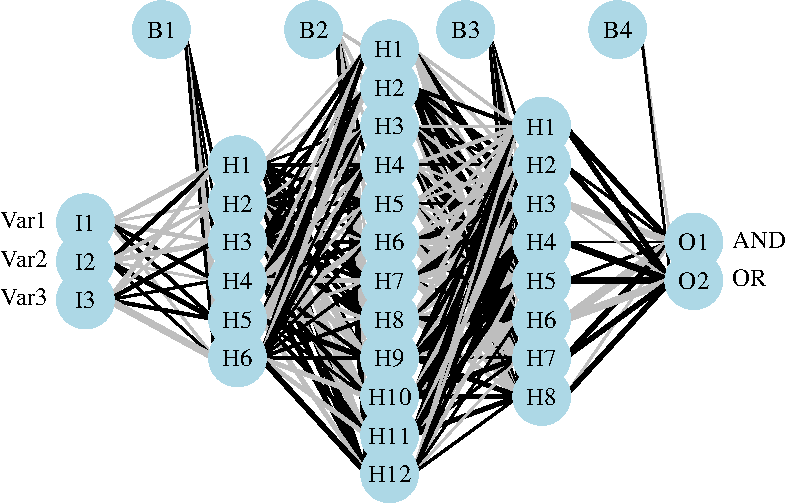
\includegraphics[width=0.7\linewidth]{regression_903-visualization_nn_files/figure-latex/unnamed-chunk-10-1} \end{center}

\hypertarget{color-coding-the-input-layer}{%
\section{color coding the input layer}\label{color-coding-the-input-layer}}

The color vector argument (circle.col) for the nodes was changed to allow a separate color vector for the input layer.

The following example shows how this can be done using relative importance of the input variables to color-code the first layer.

\begin{Shaded}
\begin{Highlighting}[]
\CommentTok{# example showing use of separate colors for input layer}
\CommentTok{# color based on relative importance using 'gar.fun'}
 
\CommentTok{##}
\CommentTok{#create input data}
\NormalTok{seed.val<-}\DecValTok{3}
\KeywordTok{set.seed}\NormalTok{(seed.val)}
  
\NormalTok{num.vars<-}\DecValTok{8}
\NormalTok{num.obs<-}\DecValTok{1000}
  
\CommentTok{#input variables}
\KeywordTok{library}\NormalTok{(clusterGeneration)}
\NormalTok{cov.mat<-}\KeywordTok{genPositiveDefMat}\NormalTok{(num.vars,}\DataTypeTok{covMethod=}\KeywordTok{c}\NormalTok{(}\StringTok{"unifcorrmat"}\NormalTok{))}\OperatorTok{$}\NormalTok{Sigma}
\NormalTok{rand.vars<-}\KeywordTok{mvrnorm}\NormalTok{(num.obs,}\KeywordTok{rep}\NormalTok{(}\DecValTok{0}\NormalTok{,num.vars),}\DataTypeTok{Sigma=}\NormalTok{cov.mat)}
  
\CommentTok{# output variables}
\NormalTok{parms<-}\KeywordTok{runif}\NormalTok{(num.vars,}\OperatorTok{-}\DecValTok{10}\NormalTok{,}\DecValTok{10}\NormalTok{)}
\NormalTok{y1<-rand.vars }\OperatorTok\StringTok{ }\KeywordTok{matrix}\NormalTok{(parms) }\OperatorTok{+}\StringTok{ }\KeywordTok{rnorm}\NormalTok{(num.obs,}\DataTypeTok{sd=}\DecValTok{20}\NormalTok{)}
 
\CommentTok{# final datasets}
\NormalTok{rand.vars<-}\KeywordTok{data.frame}\NormalTok{(rand.vars)}
\NormalTok{resp<-}\KeywordTok{data.frame}\NormalTok{(y1)}
\KeywordTok{names}\NormalTok{(resp)<-}\StringTok{'Y1'}
\NormalTok{dat.in <-}\StringTok{ }\KeywordTok{data.frame}\NormalTok{(resp,rand.vars)}
 
\CommentTok{##}
\CommentTok{# create model}
\KeywordTok{library}\NormalTok{(nnet)}
\NormalTok{mod1 <-}\StringTok{ }\KeywordTok{nnet}\NormalTok{(rand.vars,resp,}\DataTypeTok{data=}\NormalTok{dat.in,}\DataTypeTok{size=}\DecValTok{10}\NormalTok{,}\DataTypeTok{linout=}\NormalTok{T)}
\CommentTok{#> # weights:  101}
\CommentTok{#> initial  value 844959.580478 }
\CommentTok{#> iter  10 value 543616.101824}
\CommentTok{#> iter  20 value 479986.887846}
\CommentTok{#> iter  30 value 465607.784054}
\CommentTok{#> iter  40 value 454237.073298}
\CommentTok{#> iter  50 value 445032.412421}
\CommentTok{#> iter  60 value 433191.158624}
\CommentTok{#> iter  70 value 426321.161292}
\CommentTok{#> iter  80 value 424900.966883}
\CommentTok{#> iter  90 value 423816.437605}
\CommentTok{#> iter 100 value 422064.114812}
\CommentTok{#> final  value 422064.114812 }
\CommentTok{#> stopped after 100 iterations}
 
\CommentTok{##}
\CommentTok{# relative importance function}
\KeywordTok{library}\NormalTok{(devtools)}
\KeywordTok{source_url}\NormalTok{(}\StringTok{'https://gist.github.com/fawda123/6206737/raw/2e1bc9cbc48d1a56d2a79dd1d33f414213f5f1b1/gar_fun.r'}\NormalTok{)}
\CommentTok{#> SHA-1 hash of file is 9faa58824c46956c3ff78081696290d9b32d845f}
 
\CommentTok{# relative importance of input variables for Y1}
\NormalTok{rel.imp <-}\StringTok{ }\KeywordTok{gar.fun}\NormalTok{(}\StringTok{'Y1'}\NormalTok{,mod1,}\DataTypeTok{bar.plot=}\NormalTok{F)}\OperatorTok{$}\NormalTok{rel.imp}
 
\CommentTok{#color vector based on relative importance of input values}
\NormalTok{cols<-}\KeywordTok{colorRampPalette}\NormalTok{(}\KeywordTok{c}\NormalTok{(}\StringTok{'green'}\NormalTok{,}\StringTok{'red'}\NormalTok{))(num.vars)[}\KeywordTok{rank}\NormalTok{(rel.imp)]}
 
\CommentTok{##}
\CommentTok{#plotting function}
\KeywordTok{source_url}\NormalTok{(}\StringTok{'https://gist.githubusercontent.com/fawda123/7471137/raw/466c1474d0a505ff044412703516c34f1a4684a5/nnet_plot_update.r'}\NormalTok{)}
\CommentTok{#> SHA-1 hash of file is 74c80bd5ddbc17ab3ae5ece9c0ed9beb612e87ef}
  
\CommentTok{#plot model with new color vector}
\CommentTok{#separate colors for input vectors using a list for 'circle.col'}
\KeywordTok{plot}\NormalTok{(mod1,}\DataTypeTok{circle.col=}\KeywordTok{list}\NormalTok{(cols,}\StringTok{'lightblue'}\NormalTok{))}
\end{Highlighting}
\end{Shaded}

\begin{center}\includegraphics[width=0.7\linewidth]{regression_903-visualization_nn_files/figure-latex/unnamed-chunk-11-1} \end{center}

\hypertarget{regression-boston-nnet}{%
\chapter{Regression Boston nnet}\label{regression-boston-nnet}}

\begin{Shaded}
\begin{Highlighting}[]
\CommentTok{###}
\CommentTok{### prepare data}
\CommentTok{###}
\KeywordTok{library}\NormalTok{(mlbench)}
\KeywordTok{data}\NormalTok{(BostonHousing)}
 
\CommentTok{# inspect the range which is 1-50}
\KeywordTok{summary}\NormalTok{(BostonHousing}\OperatorTok{$}\NormalTok{medv)}
\CommentTok{#>    Min. 1st Qu.  Median    Mean 3rd Qu.    Max. }
\CommentTok{#>     5.0    17.0    21.2    22.5    25.0    50.0}
 
 
\CommentTok{##}
\CommentTok{## model linear regression}
\CommentTok{##}
 
\NormalTok{lm.fit <-}\StringTok{ }\KeywordTok{lm}\NormalTok{(medv }\OperatorTok{~}\StringTok{ }\NormalTok{., }\DataTypeTok{data=}\NormalTok{BostonHousing)}
 
\NormalTok{lm.predict <-}\StringTok{ }\KeywordTok{predict}\NormalTok{(lm.fit)}
 
\CommentTok{# mean squared error: 21.89483}
\KeywordTok{mean}\NormalTok{((lm.predict }\OperatorTok{-}\StringTok{ }\NormalTok{BostonHousing}\OperatorTok{$}\NormalTok{medv)}\OperatorTok{^}\DecValTok{2}\NormalTok{) }
\CommentTok{#> [1] 21.9}
 
\KeywordTok{plot}\NormalTok{(BostonHousing}\OperatorTok{$}\NormalTok{medv, lm.predict,}
    \DataTypeTok{main=}\StringTok{"Linear regression predictions vs actual"}\NormalTok{,}
    \DataTypeTok{xlab=}\StringTok{"Actual"}\NormalTok{)}
\end{Highlighting}
\end{Shaded}

\begin{center}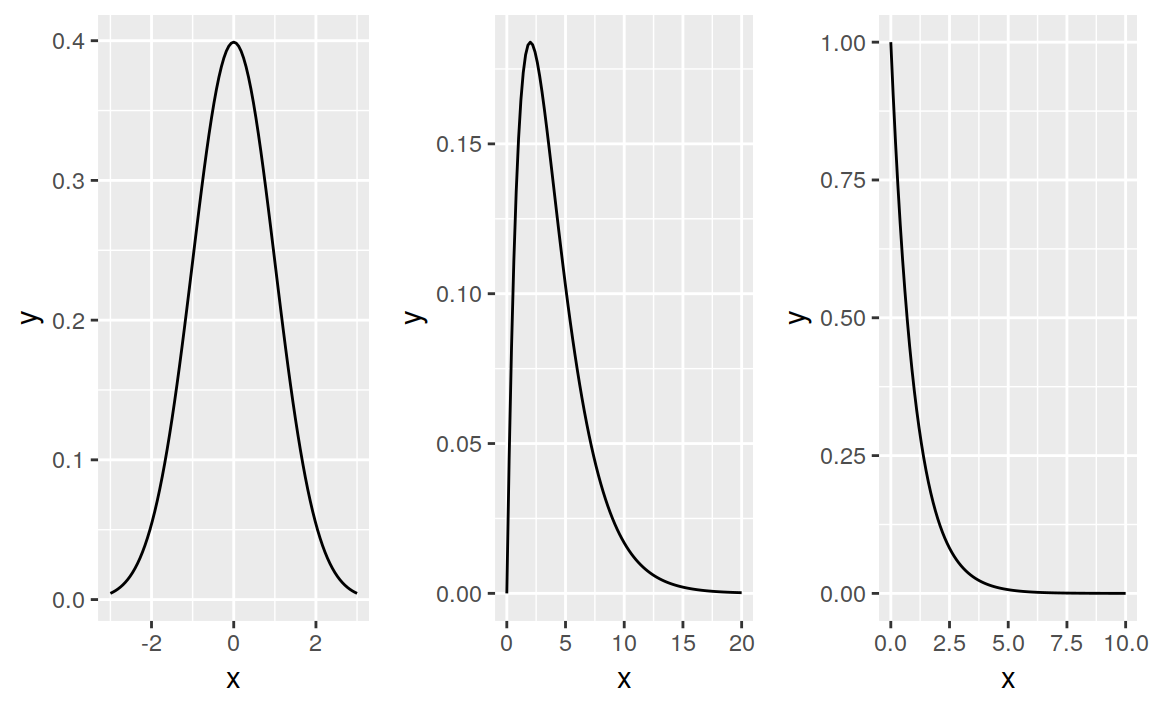
\includegraphics[width=0.7\linewidth]{regression_921-nn_lm_vs_nn_files/figure-latex/unnamed-chunk-2-1} \end{center}

\begin{Shaded}
\begin{Highlighting}[]
\CommentTok{##}
\CommentTok{## model neural network}
\CommentTok{##}
\KeywordTok{require}\NormalTok{(nnet)}
\CommentTok{#> Loading required package: nnet}
 
\CommentTok{# scale inputs: divide by 50 to get 0-1 range}
\NormalTok{nnet.fit <-}\StringTok{ }\KeywordTok{nnet}\NormalTok{(medv}\OperatorTok{/}\DecValTok{50} \OperatorTok{~}\StringTok{ }\NormalTok{., }\DataTypeTok{data=}\NormalTok{BostonHousing, }\DataTypeTok{size=}\DecValTok{2}\NormalTok{) }
\CommentTok{#> # weights:  31}
\CommentTok{#> initial  value 17.039194 }
\CommentTok{#> iter  10 value 13.754559}
\CommentTok{#> iter  20 value 13.537235}
\CommentTok{#> iter  30 value 13.537183}
\CommentTok{#> iter  40 value 13.530522}
\CommentTok{#> final  value 13.529736 }
\CommentTok{#> converged}
 
\CommentTok{# multiply 50 to restore original scale}
\NormalTok{nnet.predict <-}\StringTok{ }\KeywordTok{predict}\NormalTok{(nnet.fit)}\OperatorTok{*}\DecValTok{50} 
 
\CommentTok{# mean squared error: 16.40581}
\KeywordTok{mean}\NormalTok{((nnet.predict }\OperatorTok{-}\StringTok{ }\NormalTok{BostonHousing}\OperatorTok{$}\NormalTok{medv)}\OperatorTok{^}\DecValTok{2}\NormalTok{) }
\CommentTok{#> [1] 66.8}
 
\KeywordTok{plot}\NormalTok{(BostonHousing}\OperatorTok{$}\NormalTok{medv, nnet.predict,}
    \DataTypeTok{main=}\StringTok{"Neural network predictions vs actual"}\NormalTok{,}
    \DataTypeTok{xlab=}\StringTok{"Actual"}\NormalTok{)}
\end{Highlighting}
\end{Shaded}

\begin{center}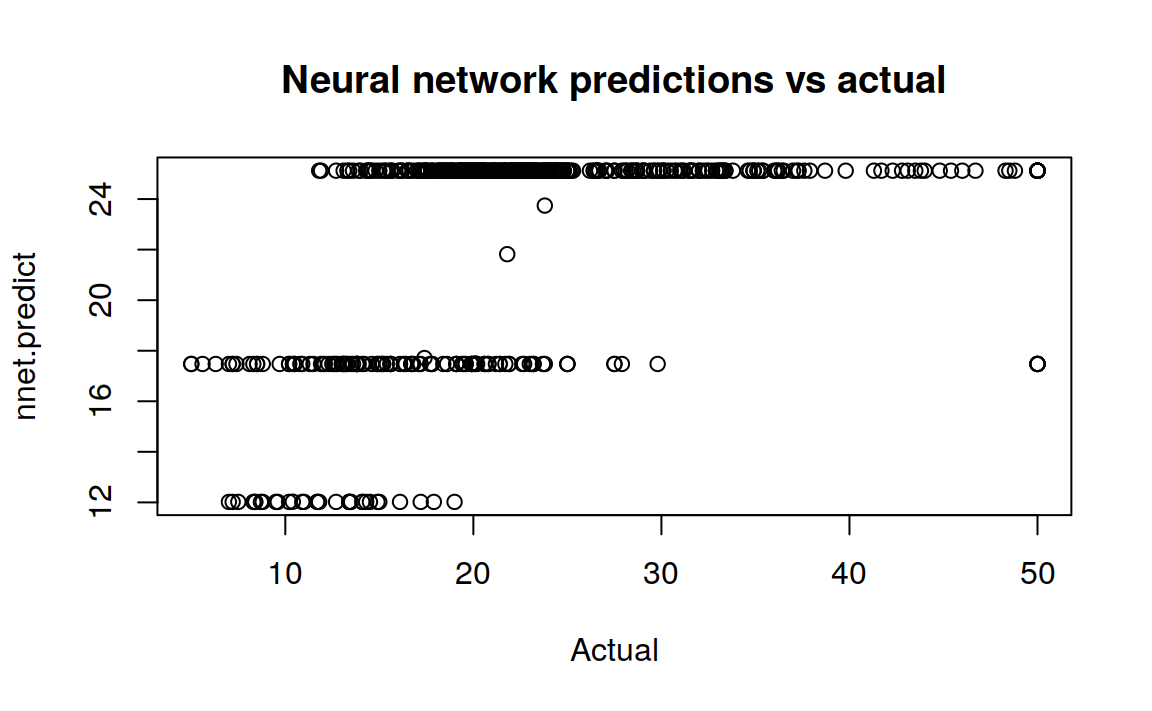
\includegraphics[width=0.7\linewidth]{regression_921-nn_lm_vs_nn_files/figure-latex/unnamed-chunk-3-1} \end{center}

\hypertarget{neural-network}{%
\section{Neural Network}\label{neural-network}}

Now, let's use the function train() from the package caret to optimize the neural network hyperparameters decay and size, Also, caret performs resampling to give a better estimate of the error. In this case we scale linear regression by the same value, so the error statistics are directly comparable.

\begin{Shaded}
\begin{Highlighting}[]
 \KeywordTok{library}\NormalTok{(mlbench)}
 \KeywordTok{data}\NormalTok{(BostonHousing)}
 
\KeywordTok{require}\NormalTok{(caret)}
\CommentTok{#> Loading required package: caret}
\CommentTok{#> Loading required package: lattice}
\CommentTok{#> Loading required package: ggplot2}
\CommentTok{#> Registered S3 methods overwritten by 'ggplot2':}
\CommentTok{#>   method         from }
\CommentTok{#>   [.quosures     rlang}
\CommentTok{#>   c.quosures     rlang}
\CommentTok{#>   print.quosures rlang}
 
\NormalTok{mygrid <-}\StringTok{ }\KeywordTok{expand.grid}\NormalTok{(}\DataTypeTok{.decay=}\KeywordTok{c}\NormalTok{(}\FloatTok{0.5}\NormalTok{, }\FloatTok{0.1}\NormalTok{), }\DataTypeTok{.size=}\KeywordTok{c}\NormalTok{(}\DecValTok{4}\NormalTok{,}\DecValTok{5}\NormalTok{,}\DecValTok{6}\NormalTok{))}
\NormalTok{nnetfit <-}\StringTok{ }\KeywordTok{train}\NormalTok{(medv}\OperatorTok{/}\DecValTok{50} \OperatorTok{~}\StringTok{ }\NormalTok{., }\DataTypeTok{data=}\NormalTok{BostonHousing, }\DataTypeTok{method=}\StringTok{"nnet"}\NormalTok{, }\DataTypeTok{maxit=}\DecValTok{1000}\NormalTok{, }\DataTypeTok{tuneGrid=}\NormalTok{mygrid, }\DataTypeTok{trace=}\NormalTok{F) }
\KeywordTok{print}\NormalTok{(nnetfit)}
\CommentTok{#> Neural Network }
\CommentTok{#> }
\CommentTok{#> 506 samples}
\CommentTok{#>  13 predictor}
\CommentTok{#> }
\CommentTok{#> No pre-processing}
\CommentTok{#> Resampling: Bootstrapped (25 reps) }
\CommentTok{#> Summary of sample sizes: 506, 506, 506, 506, 506, 506, ... }
\CommentTok{#> Resampling results across tuning parameters:}
\CommentTok{#> }
\CommentTok{#>   decay  size  RMSE    Rsquared  MAE   }
\CommentTok{#>   0.1    4     0.0835  0.787     0.0571}
\CommentTok{#>   0.1    5     0.0822  0.794     0.0565}
\CommentTok{#>   0.1    6     0.0799  0.806     0.0544}
\CommentTok{#>   0.5    4     0.0908  0.757     0.0626}
\CommentTok{#>   0.5    5     0.0900  0.761     0.0624}
\CommentTok{#>   0.5    6     0.0895  0.763     0.0622}
\CommentTok{#> }
\CommentTok{#> RMSE was used to select the optimal model using the smallest value.}
\CommentTok{#> The final values used for the model were size = 6 and decay = 0.1.}
\end{Highlighting}
\end{Shaded}

\begin{verbatim}
506 samples
 13 predictors
 
No pre-processing
Resampling: Bootstrap (25 reps) 
 
Summary of sample sizes: 506, 506, 506, 506, 506, 506, ... 
 
Resampling results across tuning parameters:
 
  size  decay  RMSE    Rsquared  RMSE SD  Rsquared SD
  4     0.1    0.0852  0.785     0.00863  0.0406     
  4     0.5    0.0923  0.753     0.00891  0.0436     
  5     0.1    0.0836  0.792     0.00829  0.0396     
  5     0.5    0.0899  0.765     0.00858  0.0399     
  6     0.1    0.0835  0.793     0.00804  0.0318     
  6     0.5    0.0895  0.768     0.00789  0.0344   
\end{verbatim}

\hypertarget{linear-regression}{%
\section{Linear Regression}\label{linear-regression}}

\begin{Shaded}
\begin{Highlighting}[]
\NormalTok{ lmfit <-}\StringTok{ }\KeywordTok{train}\NormalTok{(medv}\OperatorTok{/}\DecValTok{50} \OperatorTok{~}\StringTok{ }\NormalTok{., }\DataTypeTok{data=}\NormalTok{BostonHousing, }\DataTypeTok{method=}\StringTok{"lm"}\NormalTok{) }
 \KeywordTok{print}\NormalTok{(lmfit)}
\CommentTok{#> Linear Regression }
\CommentTok{#> }
\CommentTok{#> 506 samples}
\CommentTok{#>  13 predictor}
\CommentTok{#> }
\CommentTok{#> No pre-processing}
\CommentTok{#> Resampling: Bootstrapped (25 reps) }
\CommentTok{#> Summary of sample sizes: 506, 506, 506, 506, 506, 506, ... }
\CommentTok{#> Resampling results:}
\CommentTok{#> }
\CommentTok{#>   RMSE    Rsquared  MAE   }
\CommentTok{#>   0.0988  0.726     0.0692}
\CommentTok{#> }
\CommentTok{#> Tuning parameter 'intercept' was held constant at a value of TRUE}
\end{Highlighting}
\end{Shaded}

\begin{verbatim}
506 samples
 13 predictors
 
No pre-processing
Resampling: Bootstrap (25 reps) 
 
Summary of sample sizes: 506, 506, 506, 506, 506, 506, ... 
 
Resampling results
 
  RMSE    Rsquared  RMSE SD  Rsquared SD
  0.0994  0.703     0.00741  0.0389    
\end{verbatim}

A tuned neural network has a RMSE of 0.0835 compared to linear regression's RMSE of 0.0994.

\bibliography{book.bib,packages.bib}


\end{document}
